\chapter{HPC ranking of big performance tableaux}
\label{sec:11}

\abstract*{ The sparse outranking digraph, introduced inn Chapter~\ref{sec:9} is suitable for tackling the ranking of big multiple criteria performance tableaux with thausands or millions of records. To effectively compute rankings from performance tableaux of these sizes, we propose in this chapter a collection of C-compiled and optimised \Digraph modules that may be run on HPC equipement as available, for instance at the University of Luxembourg.}

\abstract{ The sparse outranking digraph, introduced inn Chapter~\ref{sec:9} is suitable for tackling the ranking of big multiple criteria performance tableaux with thausands or millions of records. To effectively compute rankings from performance tableaux of these sizes, we propose in this chapter a collection of C-compiled and optimised \Digraph modules that may be run on HPC equipement as available, for instance at the University of Luxembourg.}

\section{C-compiled Python modules}
\label{sec:11.1}

The \Digraph collection provides cythonized \footnote{\Cython C-extension for Python, https://cython.org/}, i.e. C-compiled and optimised versions of the main python modules for tackling multiple criteria decision problems facing very large sets of decision alternatives ( $> 10000$ ). Such problems appear usually with a combinatorial organisation of the potential decision alternatives, as is frequently the case in bioinformatics for instance. If HPC facilities with nodes supporting numerous cores ($> 20$) and big RAM ($>$ 50GB) are available, ranking up to several millions of alternatives becomes effectively tractable (see \citep{BIS-2016}).

Four cythonized \Digraph modules, prefixed with the letter \texttt{c} and taking a \texttt{pyx} extension, are provided with their corresponding setup tools in the \texttt{cython} directory of the \Digraph resources, namely:
\begin{itemize}[topsep=1pt]
\item[] \texttt{cRandPerfTabs.pyx},
\item[] \texttt{cIntegerOutrankingDigraphs.pyx},
\item[] \texttt{cIntegerSortingDigraphs.pyx}, and
\item[] \texttt{cSparseIntegerOutrankingDigraphs.pyx}.
\end{itemize}

Their automatic compilation and installation, alongside the standard \Digraph python3 modules, requires the \emph{cython} compiler:

\texttt{...\$ python3 -m pip install cython}

\noindent and a C compiler:

\texttt{...\$ sudo apt install gcc} on Ubuntu, for instance.

These cythonized modules, specifically designed for being run on HPC clusters, require the Unix \emph{forking} start method of subprocesses and therefore, due to forking problems on Mac OS platforms, may only operate safely on Linux platforms (see start methods of the \href{https://docs.python.org/3/library/multiprocessing.html#contexts-and-start-methods}{Python multiprocessing library}).

\section{Big Data performance tableaux}
\label{sec:11.2}

In order to efficiently type the C variables, the \texttt{cRandPerfTabs} module\index{cRandPerfTabs@\texttt{cRandPerfTabs} module} provides the root \texttt{cPerformanceTableau} class\index{cPerformanceTableau@\texttt{cPerformanceTableau} class}, but, with \emph{integer} action keys, \emph{float} performance evaluations, \emph{integer} criteria weights and \emph{float} discrimination thresholds. And, to limit as much as possible memory occupation of class instances, all the usual verbose comments are dropped from the description of the \texttt{actions} and \texttt{criteria} dictionaries. A random instance may be generated with the  \texttt{cRandomPerformanceTableau} class\index{cRandomPerformanceTableau@\texttt{cRandomPerformanceTableau} class}:
\begin{lstlisting}[caption={Big data performance tableau format},label=list:11.1,basicstyle=\ttfamily\scriptsize]
>>> from cRandPerfTabs import cRandomPerformanceTableau
>>> t = cRandomPerformanceTableau(numberOfActions=4,\
...                               numberOfCriteria=2)
>>> t
  *------- PerformanceTableau instance description ------*
    Instance class   : cRandomPerformanceTableau
    Seed             : None
    Instance name    : cRandomperftab
    Actions          : 4
    Criteria         : 2
    Attributes       : ['randomSeed', 'name', 'actions',
                        'criteria', 'evaluation', 'weightPreorder']
>>> t.actions
   OrderedDict([(1, {'name': '#1'}), (2, {'name': '#2'}),
		(3, {'name': '#3'}), (4, {'name': '#4'})])
>>> t.criteria
   OrderedDict([
   ('g1', {'name': 'RandomPerformanceTableau() instance',
	       'thresholds': {'ind': (10.0, 0.0),
			       'pref': (20.0, 0.0),
			       'veto': (80.0, 0.0)},
	       'scale': (0.0, 100.0),
	       'weight': 1,
	       'preferenceDirection': 'max'}),
   ('g2', {'name': 'RandomPerformanceTableau() instance',
	       'thresholds': {'ind': (10.0, 0.0),
			       'pref': (20.0, 0.0),
			       'veto': (80.0, 0.0)},
	       'scale': (0.0, 100.0),
	       'weight': 1,
	       'preferenceDirection': 'max'})])
>>> t.evaluation
  {'g1': {1: 35.17, 2: 56.4, 3: 1.94, 4: 5.51},
   'g2': {1: 95.12, 2: 90.54, 3: 51.84, 4: 15.42}}
>>> t.showPerformanceTableau()
	Criteria |  'g1'    'g2'   
	Actions  |    1       1    
	---------|---------------
	   '#1'  |  91.18   90.42  
	   '#2'  |  66.82   41.31  
	   '#3'  |  35.76   28.86  
	   '#4'  |   7.78   37.64  
\end{lstlisting}

Several methods for converting from the Big Data model to the standard model and vice versa are provided by the \texttt{cPerformanceTableau} class.\index{convert2Standard@\texttt{convert2Standard()}}\index{convertWeight2Decimal@\texttt{convertWeight2Decimal()}}\index{convertEvaluation2Decimal@\texttt{convertEvaluation2Decimal()}}
\begin{lstlisting}   
>>> t1 = t.convert2Standard()
>>> t1.convertWeight2Decimal()
>>> t1.convertEvaluation2Decimal()
>>> t1
  *------- PerformanceTableau instance description ------*
   Instance class   : PerformanceTableau
   Seed             : None
   Instance name    : std_cRandomperftab
   Actions          : 4
   Criteria         : 2
   Attributes       : ['name', 'actions', 'criteria',
                       'weightPreorder', 'evaluation',
                       'randomSeed']
\end{lstlisting}

\section{C-implemented integer-valued outranking digraphs}
\label{sec:11.3}

The C compiled version of the \texttt{BipolarOutrankingDigraph} class takes integer $r$-characteristic values.\index{cIntegerOutrankingDigraphs@\texttt{cIntegerOutrankingDigraphs} module}\index{IntegerBipolarOutrankingDigraph@\texttt{IntegerBipolarOutrankingDigraph} class}
\begin{lstlisting}[caption={Constructing big bipolar-valued outranking digraphs},label=list:11.2]
>>> from cRandPerfTabs import cRandomPerformanceTableau
>>> t = cRandomPerformanceTableau(numberOfActions=1000,\
...                               numberOfCriteria=2,seed=100)
>>> from cIntegerOutrankingDigraphs import\
...                 IntegerBipolarOutrankingDigraph
>>> g = IntegerBipolarOutrankingDigraph(t,\
...                 Threading=True, nbrCores=4)
>>> g
  *------- Object instance description ------*
   Instance class   : IntegerBipolarOutrankingDigraph
   Instance name    : rel_cRandomperftab
   Actions          : 1000
   Criteria         : 2
   Size             : 460795
   Determinateness  : 55.975
   Valuation domain : {'min': -2, 'med': 0, 'max': 2,
                       'hasIntegerValuation': True}
   ----  Constructor run times (in sec.) ----
   Total time       : 4.10093
   Data input       : 0.00955
   Compute relation : 3.33437
   Gamma sets       : 0.75699
   Size             : 465024
   Determinateness  : 56.877
   Attributes       : ['name', 'actions', 'criteria',
                       'totalWeight', 'valuationdomain',
                       'methodData', 'evaluation',
                       'order', 'runTimes', 'nbrThreads',
                       'relation', 'gamma', 'notGamma']
\end{lstlisting}

On a classical intel-i7 equipped PC with four single threaded cores, the \texttt{Inte\-ger\-BipolarOutrankingDigraph} class constructor takes about four seconds for computing a \emph{million} pairwise outranking characteristic values (see List.~\vref{list:11.2}). In a similar setting, the standard \texttt{BipolarOutranking\-Digraph} constructor operates more than two times slower.
\begin{lstlisting}
>>> from outrankingDigraphs import BipolarOutrankingDigraph
>>> t1 = t.convert2Standard()
>>> g1 = BipolarOutrankingDigraph(t1,\
...                Threading=True,nbrCores=4)
>>> g1
  *------- Object instance description ------*
    Instance class       : BipolarOutrankingDigraph
    Instance name        : rel_std_cRandomperftab
    Actions              : 1000
    Criteria             : 2
    Size                 : 460795
    Determinateness (%)  : 77.99
    Valuation domain     : [-1.00;1.00]
    Attributes           : ['name','actions','valuationdomain',
                            'criteria','methodData','evaluation',
                            'NA','order','runTimes','nbrThreads',
                            'relation','gamma','notGamma']
    ----  Constructor run times (in sec.) ----
    Total time           : 14.92166
    Data input           : 0.01506
    Compute relation     : 13.51562
    Gamma sets           : 1.39096
    Threads              : 4
\end{lstlisting}

By far, most of the run time is in each case needed for computing the individual pairwise outranking characteristic values: $4.10$ sec. versus $14.92$ sec. Notice also below the memory occupations --about 108MB for \texttt{g} and 216MB for \texttt{g1}-- of both outranking digraph instances.\index{digraphsTools@\texttt{digraphsTools} module}\index{total-size@\texttt{total\_size()}}
\begin{lstlisting}
>>> from digraphsTools import total_size
>>> total_size(g)
    107503580
>>> total_size(g1)
    211519995
>>> total_size(g1.relation)/total_size(g1)
    0.67
>>> total_size(g1.gamma)/total_size(g1)
    0.23
\end{lstlisting}

The standard \texttt{Decimal} valued \texttt{BipolarOutrankingDigraph} instance \texttt{g1} thus nearly doubles the memory occupation of the corresponding \texttt{IntegerBipo\-larOutrankingDigraph} \texttt{g} instance (see Line 3 and 5 above). $90\%$ of this memory occupation is due to the \texttt{g1.relation} ($67\%$) and the \texttt{g1.gamma} ($23\%$) dictionaries. And these ratios quadratically grow with the digraph order. To limit the object sizes for really big outranking digraphs, we need to abandon the complete implementation of adjacency tables and gamma functions.

\section{The sparse implementation of big outranking digraphs}
\label{sec:11.4}

The idea is to first decompose the complete outranking relation into an ordered collection of equivalent quantile performance classes. Let us consider for this illustration a random performance tableau with 100 decision alternatives evaluated on 7 criteria.
\begin{lstlisting}
>>> from cRandPerfTabs import cRandomPerformanceTableau
>>> t = cRandomPerformanceTableau(numberOfActions=100,\
...                       numberOfCriteria=7,seed=100)
\end{lstlisting}

The \texttt{cSparseIntegerOutrankingDigraphs} module\index{cSparseIntegerOutrankingDigraphs@\texttt{cSparseIntegerOutranking\-Digraphs} module} provides the \texttt{Spar\-seIntegerOutrankingDigraph} class\index{SparseIntegerOutrankingDigraph@\texttt{SparseIntegerOutrankingDigraph} class} for sorting the $100$ decision alternatives into overlapping quartile classes and rank all $100$ with respect to the average quantile limits.
\begin{lstlisting}[caption={Constructing the sparse integer outranking digraph},label=list:11.3]
>>> from cSparseIntegerOutrankingDigraphs import\
...                    SparseIntegerOutrankingDigraph
>>> sg = SparseIntegerOutrankingDigraph(t,quantiles=4)
>>> sg
  *----- Object instance description --------------*
   Instance class    : SparseIntegerOutrankingDigraph
   Instance name     : cRandomperftab_mp
   Actions           : 100
   Criteria          : 7
   Sorting by        : 4-Tiling
   Ordering strategy : average
   Ranking rule      : Copeland
   Components        : 6
   Minimal order     : 1
   Maximal order     : 35
   Average order     : 16.7
   fill rate         : 24.970%
  *----  Constructor run times (in sec.) ----
   Nbr of threads    : 1
   Total time        : 0.08212
   QuantilesSorting  : 0.01481
   Preordering       : 0.00022
   Decomposing       : 0.06707
   Ordering          : 0.00000
   Attributes       : ['runTimes', 'name', 'actions',
       'criteria', 'evaluation', 'order', 'dimension',
       'sortingParameters', 'nbrOfCPUs',
       'valuationdomain', 'profiles', 'categories',
       'sorting', 'minimalComponentSize',
       'decomposition', 'nbrComponents', 'nd',
       'components', 'fillRate',
       'maximalComponentSize', 'componentRankingRule',
       'boostedRanking']
\end{lstlisting}

We obtain in this example here a decomposition into 6 linearly ordered components with a maximal component size of 35 for component \texttt{c3}.

\begin{lstlisting}
>>> sg.showDecomposition()
 *--- quantiles decomposition in decreasing order---*
  c1. ]0.75-1.00] : [3,22,24,34,41,44,50,53,56,62,93]
  c2. ]0.50-1.00] : [7,29,43,58,63,81,96]
  c3. ]0.50-0.75] : [1,2,5,8,10,11,20,21,25,28,30,33,
                     35,36,45,48,57,59,61,65,66,68,70,
                     71,73,76,82,85,89,90,91,92,94,95,97]
  c4. ]0.25-0.75] : [17,19,26,27,40,46,55,64,69,87,98,100]
  c5. ]0.25-0.50] : [4,6,9,12,13,14,15,16,18,23,31,32,
                     37,38,39,42,47,49,51,52,54,60,67,72,
                     74,75,77,78,80,86,88,99]
  c6. ]<-0.25]    : [79,83,84]
\end{lstlisting}

A restricted outranking relation is stored for each component with more than one alternative. The showRelationMap() prints out below the relation map of the sparse digraph \texttt{sg} for the 75 first-ranked alternatives. (see Fig.~\vref{fig:11.1}):
\begin{lstlisting}
>>> sg.showRelationMap(toIndex=75)
\end{lstlisting}  
\begin{figure}[ht]
\sidecaption[t]
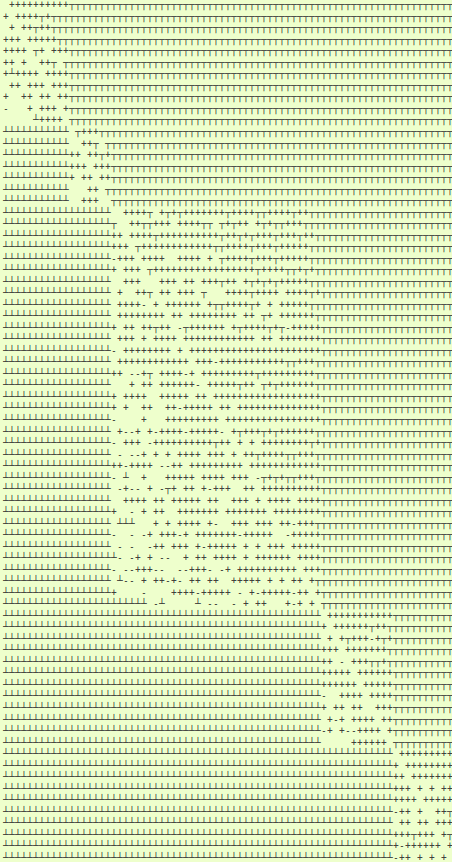
\includegraphics[width=7cm]{Figures/11-1-sparseRelationMap.png}
\caption[Sparse quartiles-sorting decomposed outranking relation]{Sparse quartiles-sorting decomposed outranking relation (extract). Legend: \emph{outranking} for certain ($\top$); \emph{outranked} for certain ($\bot$); more or less \emph{outranking} ($+$); more or less \emph{outranked} ($-$); \emph{indeterminate}}
\label{fig:11.1}       % Give a unique label
\end{figure}
%\clearpage

With a fill rate of $25\%$, the memory occupation of this sparse outranking digraph \texttt{sg} instance takes now only $769$kB, compared to the $1.7$MB required by a corresponding standard \texttt{BipolarOutrankingDigraph} instance (see List.\vref{list:11.3}).
\begin{lstlisting}
>>> print('%.0fkB' % (total_size(sg)/1024) )
    769kB
\end{lstlisting}

For sparse outranking digraphs, the adjacency table is implemented as a dynamic \texttt{relation()} function instead of a double dictionary.
\begin{lstlisting}[caption={The \texttt{relation()} function of a sparse outranking digraph},label=list:11.4,basicstyle=\ttfamily\scriptsize]
   def relation(self, int x, int y):
       """
       *Parameters*:
           * x (int action key),
           * y (int action key).
       Dynamic construction of the global outranking
       characteristic function *r(x S y)*.
       """
       cdef int Min, Med, Max, rx, ry
       Min = self.valuationdomain['min']
       Med = self.valuationdomain['med']
       Max = self.valuationdomain['max']
       if x == y:
           return Med
       cx = self.actions[x]['component']
       cy = self.actions[y]['component']
       #print(self.components)
       rx = self.components[cx]['rank']
       ry = self.components[cy]['rank']
       if rx == ry:
           try:
               rxpg = self.components[cx]['subGraph'].relation
               return rxpg[x][y]
           except AttributeError:
               componentRanking = self.components[cx]['componentRanking']
               if componentRanking.index(x) < componentRanking.index(x):
                   return Max
               else:
                   return Min
       elif rx > ry:
           return Min
       else:
           return Max
\end{lstlisting}

\section{Quantiles ranking of big performance tableaux}
\label{sec:11.4}

The \texttt{boostedRanking} attribute of the sparse outranking digraph \texttt{sg} contains the global linear ranking of the 100 decision alternatives. This ranking is computed by locally ranking the individual 6 components with the \Copeland rule (see List.~\vref{list:11.3} Lines 12 and 33).
\begin{lstlisting}
>>> sg.boostedRanking
  [22, 53, 3, 34, 56, 62, 24, 44, 50, 93, 41, 63, 29, 58,
   96, 7, 43, 81, 91, 35, 25, 76, 66, 65, 8, 10, 1, 11, 61,
   30, 48, 45, 68, 5, 89, 57, 59, 85, 82, 73, 33, 94, 70,
   97, 20, 92, 71, 90, 95, 21, 28, 2, 36, 87, 40, 98, 46, 55,
   100, 64, 17, 26, 27, 19, 69, 6, 38, 4, 37, 60, 31, 77, 78,
   47, 99, 18, 12, 80, 54, 88, 39, 9, 72, 86, 42, 13, 23, 67,
   52, 15, 32, 49, 51, 74, 16, 14, 75, 79, 83, 84]
\end{lstlisting}

When actually computing linear rankings of the complete set of alternatives, the local outranking relations per component are of no practical usage, and we may furthermore reduce the memory occupation of the resulting digraph by:
\begin{enumerate}[topsep=1pt]
\item refining the ordering of the quantile classes by taking into account how well an alternative is outranking the lower limit of its quantile class, respectively the upper limit of its quantile class is \emph{not} outranking the alternative;
\item dropping the local outranking digraphs and keeping for each component only a locally ranked list of alternatives.
\end{enumerate}

We provide therefore the \texttt{cQuantilesRankingDigraph} class\index{cQuantilesRankingDigraph@\texttt{cQuantilesRankingDigraph} class} from the \texttt{cSparseIntegerOutrankingDigraphs} module.
\begin{lstlisting}[caption={Ranking the sparse integer outranking digraph},label=list:11.5]
>>> from cSparseIntegerOutrankingDigraphs import\
...           cQuantilesRankingDigraph
>>> qr = cQuantilesRankingDigraph(t,4)
>>> qr
 *----- Object instance description --------------*
  Instance class    : cQuantilesRankingDigraph
  Instance name     : cRandomperftab_mp
  Actions           : 100
  Criteria          : 7
  Sorting by        : 4-Tiling
  Ordering strategy : optimal
  Ranking rule      : Copeland
  Components        : 47
  Minimal order     : 1
  Maximal order     : 10
  Average order     : 2.1
  fill rate         : 2.566%
 *----  Constructor run times (in sec.) ----*
  Nbr of threads    : 1
  Total time        : 0.03702
  QuantilesSorting  : 0.01785
  Preordering       : 0.00022
  Decomposing       : 0.01892
  Attributes       : ['runTimes', 'name',
  'actions', 'order', 'dimension', 'sortingParameters',
  'nbrOfCPUs','valuationdomain', 'profiles', 'categories',
  'sorting', 'minimalComponentSize','decomposition',
  'nbrComponents', 'nd', 'components', 'fillRate',
  'maximalComponentSize', 'componentRankingRule', 'boostedRanking']
\end{lstlisting}

With this \emph{optimised} quantile ordering strategy, we obtain now 47 performance equivalence classes (see List.~\vref{list:11.5} Line 13).
\begin{lstlisting}[caption={The ordered components of the sparse outranking digraph},label=list:11.6]
>>> qr.components
    OrderedDict([
    ('c01', {'rank': 1,
	     'lowQtileLimit': ']0.75',
	     'highQtileLimit': '1.00]',
	     'componentRanking': [53]}),
    ('c02', {'rank': 2,
	     'lowQtileLimit': ']0.75',
	     'highQtileLimit': '1.00]',
	     'componentRanking': [3, 23, 63, 50]}),
    ('c03', {'rank': 3,
	     'lowQtileLimit': ']0.75',
	     'highQtileLimit': '1.00]',
	     'componentRanking': [34, 44, 56, 24, 93, 41]}), 
    ...
    ...
    ...
    ('c45', {'rank': 45,
	     'lowQtileLimit': ']0.25',
	     'highQtileLimit': '0.50]',
	     'componentRanking': [49]}),
    ('c46', {'rank': 46,
	     'lowQtileLimit': ']0.25',
	     'highQtileLimit': '0.50]',
	     'componentRanking': [52, 16, 86]}),
    ('c47', {'rank': 47,
	     'lowQtileLimit': ']<',
	     'highQtileLimit': '0.25]',
	     'componentRanking': [79, 83, 84]})])
>>> print('%.0fkB' % (total_size(qr)/1024) )
    208kB
\end{lstlisting}

We observe in Listing~\vref{list:11.6} an even more considerably less voluminous memory occupation 208kB, compared to the 769kB of the \texttt{SparseIntegerOutran\-king\-Digraph} instance.

It is opportune, however, to measure the loss of quality of the resulting \Copeland ranking when working with sparse outranking digraphs.
\begin{lstlisting}[caption={Measuring the loss of quality with respect to the standard outranking digraph},label=list:11.7]
>>> from cIntegerOutrankingDigraphs import\
...                       IntegerBipolarOutrankingDigraph
>>> ig = IntegerBipolarOutrankingDigraph(t)
>>> print('Complete outranking : %+.3f'\
...    % (ig.computeOrderCorrelation(\
...             ig.computeCopelandOrder())['correlation']))
    Complete outranking : +0.747

>>> print('Sparse 4-tiling : %+.3f'\
...     % (ig.computeOrderCorrelation(\
...        list(reversed(sg.boostedRanking)))['correlation']))   
    Sparse 4-tiling          : +0.717

>>> print('Optimzed sparse 4-tiling: %+.3f'\
...  % (ig.computeOrderCorrelation(\
...     list(reversed(qr.boostedRanking)))\
...     ['correlation']))  
    Optimzed sparse 4-tiling: +0.705
\end{lstlisting}

The best ranking correlation with the pairwise outranking situations ($+0.747$) is naturally given when we apply the \Copeland rule to the standard outranking digraph (see List.~\vref{list:10.7} Line 7). When applying the same rule to the sparse 4-tiled outranking digraph, one gets a correlation of $+0.717$ (Line 12), and when applying the \Copeland rule to the optimised sparse 4-tiled digraph, we still obtain a correlation of $+0.705$ (Line 18). These optimistic results actually depend on the number of quantiles we use as well as on the given model of random performance tableau.

In case of \texttt{Random3ObjectivesPerformanceTableau} instances, for instance, we would get in a similar setting an even better standrad outranking correlation of $+0.86$, a sparse 4-tiling correlation of $+0.82$, and an optimised sparse 4-tiling correlation of $+0.81$.

\section{HPC quantiles ranking records}
\label{sec:11.5}

Following from the separability property of the $q$-tiles sorting of each action into a $q$-tiles class, the $q$-sorting algorithm may be safely split into as much threads as are multiple processing cores available for working in parallel (see Prop.~\ref{prop:9.1}). Furthermore, the ranking procedure being local to each diagonal component, these procedures may as well be safely processed in parallel threads on each component restricted outranking digraph.

Using the HPC platform of the University of Luxembourg -- https://hpc-docs.uni.lu/ \citep{UNI-2014}-- the following run times for very big ranking problems could be achieved both on:
\begin{itemize}[topsep=1pt]
\item \emph{Iris -skylake} nodes with 28 cores:\\
  (see \href{https://hpc-docs.uni.lu/systems/iris/}{https://hpc-docs.uni.lu/systems/iris}), and
\item the 3TB -bigmem \emph{Gaia-183} node with 64 cores \\
  (see \href{https://hpc.uni.lu/systems/gaia/}{https://hpc.uni.lu/systems/gaia}),
\end{itemize}
by running the cythonized Python modules in an Intel compiled virtual Python 3.6.5 environment [GCC Intel(R) 17.0.1 –enable-optimizations c++ gcc 6.3 mode] on Debian 8 Linux.

\begin{figure}[ht]
\sidecaption[t]
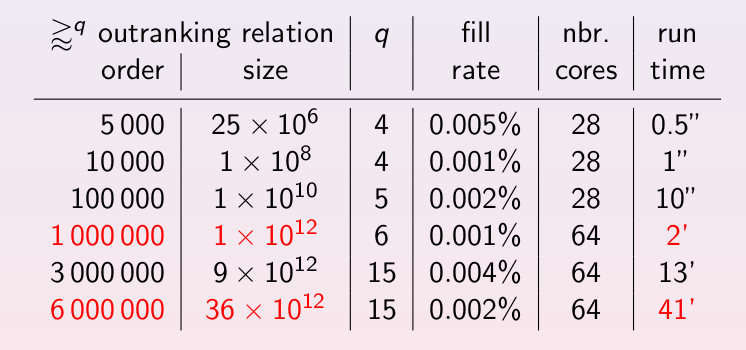
\includegraphics[width=7cm]{Figures/11-2-rankingRecords.png}
\caption[HPC-UL Ranking Performance Records (Spring 2018)]{HPC-UL Ranking Performance Records (Spring 2018). On the big memory equipped Gaia-183 node with 64 cores we were able to rank one million, resp. 6 million decision alternatives in about 2 minutes, resp. 41 minutes}
\label{fig:11.2}       % Give a unique label
\end{figure}
  
%%%%%%% The chapter bibliography
%\normallatexbib
%\clearpage
%\phantomsection
%\addcontentsline{toc}{chapter}{Chapter Bibliography}
%\chapter{HPC ranking of big performance tableaux}
\label{sec:11}

\abstract*{ The sparse outranking digraph, introduced inn Chapter~\ref{sec:9} is suitable for tackling the ranking of big multiple criteria performance tableaux with thausands or millions of records. To effectively compute rankings from performance tableaux of these sizes, we propose in this chapter a collection of C-compiled and optimised \Digraph modules that may be run on HPC equipement as available, for instance at the University of Luxembourg.}

\abstract{ The sparse outranking digraph, introduced inn Chapter~\ref{sec:9} is suitable for tackling the ranking of big multiple criteria performance tableaux with thausands or millions of records. To effectively compute rankings from performance tableaux of these sizes, we propose in this chapter a collection of C-compiled and optimised \Digraph modules that may be run on HPC equipement as available, for instance at the University of Luxembourg.}

\section{C-compiled Python modules}
\label{sec:11.1}

The \Digraph collection provides cythonized \footnote{\Cython C-extension for Python, https://cython.org/}, i.e. C-compiled and optimised versions of the main python modules for tackling multiple criteria decision problems facing very large sets of decision alternatives ( $> 10000$ ). Such problems appear usually with a combinatorial organisation of the potential decision alternatives, as is frequently the case in bioinformatics for instance. If HPC facilities with nodes supporting numerous cores ($> 20$) and big RAM ($>$ 50GB) are available, ranking up to several millions of alternatives becomes effectively tractable (see \citep{BIS-2016}).

Four cythonized \Digraph modules, prefixed with the letter \texttt{c} and taking a \texttt{pyx} extension, are provided with their corresponding setup tools in the \texttt{cython} directory of the \Digraph resources, namely:
\begin{itemize}[topsep=1pt]
\item[] \texttt{cRandPerfTabs.pyx},
\item[] \texttt{cIntegerOutrankingDigraphs.pyx},
\item[] \texttt{cIntegerSortingDigraphs.pyx}, and
\item[] \texttt{cSparseIntegerOutrankingDigraphs.pyx}.
\end{itemize}

Their automatic compilation and installation, alongside the standard \Digraph python3 modules, requires the \emph{cython} compiler:

\texttt{...\$ python3 -m pip install cython}

\noindent and a C compiler:

\texttt{...\$ sudo apt install gcc} on Ubuntu, for instance.

These cythonized modules, specifically designed for being run on HPC clusters, require the Unix \emph{forking} start method of subprocesses and therefore, due to forking problems on Mac OS platforms, may only operate safely on Linux platforms (see start methods of the \href{https://docs.python.org/3/library/multiprocessing.html#contexts-and-start-methods}{Python multiprocessing library}).

\section{Big Data performance tableaux}
\label{sec:11.2}

In order to efficiently type the C variables, the \texttt{cRandPerfTabs} module\index{cRandPerfTabs@\texttt{cRandPerfTabs} module} provides the root \texttt{cPerformanceTableau} class\index{cPerformanceTableau@\texttt{cPerformanceTableau} class}, but, with \emph{integer} action keys, \emph{float} performance evaluations, \emph{integer} criteria weights and \emph{float} discrimination thresholds. And, to limit as much as possible memory occupation of class instances, all the usual verbose comments are dropped from the description of the \texttt{actions} and \texttt{criteria} dictionaries. A random instance may be generated with the  \texttt{cRandomPerformanceTableau} class\index{cRandomPerformanceTableau@\texttt{cRandomPerformanceTableau} class}:
\begin{lstlisting}[caption={Big data performance tableau format},label=list:11.1,basicstyle=\ttfamily\scriptsize]
>>> from cRandPerfTabs import cRandomPerformanceTableau
>>> t = cRandomPerformanceTableau(numberOfActions=4,\
...                               numberOfCriteria=2)
>>> t
  *------- PerformanceTableau instance description ------*
    Instance class   : cRandomPerformanceTableau
    Seed             : None
    Instance name    : cRandomperftab
    Actions          : 4
    Criteria         : 2
    Attributes       : ['randomSeed', 'name', 'actions',
                        'criteria', 'evaluation', 'weightPreorder']
>>> t.actions
   OrderedDict([(1, {'name': '#1'}), (2, {'name': '#2'}),
		(3, {'name': '#3'}), (4, {'name': '#4'})])
>>> t.criteria
   OrderedDict([
   ('g1', {'name': 'RandomPerformanceTableau() instance',
	       'thresholds': {'ind': (10.0, 0.0),
			       'pref': (20.0, 0.0),
			       'veto': (80.0, 0.0)},
	       'scale': (0.0, 100.0),
	       'weight': 1,
	       'preferenceDirection': 'max'}),
   ('g2', {'name': 'RandomPerformanceTableau() instance',
	       'thresholds': {'ind': (10.0, 0.0),
			       'pref': (20.0, 0.0),
			       'veto': (80.0, 0.0)},
	       'scale': (0.0, 100.0),
	       'weight': 1,
	       'preferenceDirection': 'max'})])
>>> t.evaluation
  {'g1': {1: 35.17, 2: 56.4, 3: 1.94, 4: 5.51},
   'g2': {1: 95.12, 2: 90.54, 3: 51.84, 4: 15.42}}
>>> t.showPerformanceTableau()
	Criteria |  'g1'    'g2'   
	Actions  |    1       1    
	---------|---------------
	   '#1'  |  91.18   90.42  
	   '#2'  |  66.82   41.31  
	   '#3'  |  35.76   28.86  
	   '#4'  |   7.78   37.64  
\end{lstlisting}

Several methods for converting from the Big Data model to the standard model and vice versa are provided by the \texttt{cPerformanceTableau} class.\index{convert2Standard@\texttt{convert2Standard()}}\index{convertWeight2Decimal@\texttt{convertWeight2Decimal()}}\index{convertEvaluation2Decimal@\texttt{convertEvaluation2Decimal()}}
\begin{lstlisting}   
>>> t1 = t.convert2Standard()
>>> t1.convertWeight2Decimal()
>>> t1.convertEvaluation2Decimal()
>>> t1
  *------- PerformanceTableau instance description ------*
   Instance class   : PerformanceTableau
   Seed             : None
   Instance name    : std_cRandomperftab
   Actions          : 4
   Criteria         : 2
   Attributes       : ['name', 'actions', 'criteria',
                       'weightPreorder', 'evaluation',
                       'randomSeed']
\end{lstlisting}

\section{C-implemented integer-valued outranking digraphs}
\label{sec:11.3}

The C compiled version of the \texttt{BipolarOutrankingDigraph} class takes integer $r$-characteristic values.\index{cIntegerOutrankingDigraphs@\texttt{cIntegerOutrankingDigraphs} module}\index{IntegerBipolarOutrankingDigraph@\texttt{IntegerBipolarOutrankingDigraph} class}
\begin{lstlisting}[caption={Constructing big bipolar-valued outranking digraphs},label=list:11.2]
>>> from cRandPerfTabs import cRandomPerformanceTableau
>>> t = cRandomPerformanceTableau(numberOfActions=1000,\
...                               numberOfCriteria=2,seed=100)
>>> from cIntegerOutrankingDigraphs import\
...                 IntegerBipolarOutrankingDigraph
>>> g = IntegerBipolarOutrankingDigraph(t,\
...                 Threading=True, nbrCores=4)
>>> g
  *------- Object instance description ------*
   Instance class   : IntegerBipolarOutrankingDigraph
   Instance name    : rel_cRandomperftab
   Actions          : 1000
   Criteria         : 2
   Size             : 460795
   Determinateness  : 55.975
   Valuation domain : {'min': -2, 'med': 0, 'max': 2,
                       'hasIntegerValuation': True}
   ----  Constructor run times (in sec.) ----
   Total time       : 4.10093
   Data input       : 0.00955
   Compute relation : 3.33437
   Gamma sets       : 0.75699
   Size             : 465024
   Determinateness  : 56.877
   Attributes       : ['name', 'actions', 'criteria',
                       'totalWeight', 'valuationdomain',
                       'methodData', 'evaluation',
                       'order', 'runTimes', 'nbrThreads',
                       'relation', 'gamma', 'notGamma']
\end{lstlisting}

On a classical intel-i7 equipped PC with four single threaded cores, the \texttt{Inte\-ger\-BipolarOutrankingDigraph} class constructor takes about four seconds for computing a \emph{million} pairwise outranking characteristic values (see List.~\vref{list:11.2}). In a similar setting, the standard \texttt{BipolarOutranking\-Digraph} constructor operates more than two times slower.
\begin{lstlisting}
>>> from outrankingDigraphs import BipolarOutrankingDigraph
>>> t1 = t.convert2Standard()
>>> g1 = BipolarOutrankingDigraph(t1,\
...                Threading=True,nbrCores=4)
>>> g1
  *------- Object instance description ------*
    Instance class       : BipolarOutrankingDigraph
    Instance name        : rel_std_cRandomperftab
    Actions              : 1000
    Criteria             : 2
    Size                 : 460795
    Determinateness (%)  : 77.99
    Valuation domain     : [-1.00;1.00]
    Attributes           : ['name','actions','valuationdomain',
                            'criteria','methodData','evaluation',
                            'NA','order','runTimes','nbrThreads',
                            'relation','gamma','notGamma']
    ----  Constructor run times (in sec.) ----
    Total time           : 14.92166
    Data input           : 0.01506
    Compute relation     : 13.51562
    Gamma sets           : 1.39096
    Threads              : 4
\end{lstlisting}

By far, most of the run time is in each case needed for computing the individual pairwise outranking characteristic values: $4.10$ sec. versus $14.92$ sec. Notice also below the memory occupations --about 108MB for \texttt{g} and 216MB for \texttt{g1}-- of both outranking digraph instances.\index{digraphsTools@\texttt{digraphsTools} module}\index{total-size@\texttt{total\_size()}}
\begin{lstlisting}
>>> from digraphsTools import total_size
>>> total_size(g)
    107503580
>>> total_size(g1)
    211519995
>>> total_size(g1.relation)/total_size(g1)
    0.67
>>> total_size(g1.gamma)/total_size(g1)
    0.23
\end{lstlisting}

The standard \texttt{Decimal} valued \texttt{BipolarOutrankingDigraph} instance \texttt{g1} thus nearly doubles the memory occupation of the corresponding \texttt{IntegerBipo\-larOutrankingDigraph} \texttt{g} instance (see Line 3 and 5 above). $90\%$ of this memory occupation is due to the \texttt{g1.relation} ($67\%$) and the \texttt{g1.gamma} ($23\%$) dictionaries. And these ratios quadratically grow with the digraph order. To limit the object sizes for really big outranking digraphs, we need to abandon the complete implementation of adjacency tables and gamma functions.

\section{The sparse implementation of big outranking digraphs}
\label{sec:11.4}

The idea is to first decompose the complete outranking relation into an ordered collection of equivalent quantile performance classes. Let us consider for this illustration a random performance tableau with 100 decision alternatives evaluated on 7 criteria.
\begin{lstlisting}
>>> from cRandPerfTabs import cRandomPerformanceTableau
>>> t = cRandomPerformanceTableau(numberOfActions=100,\
...                       numberOfCriteria=7,seed=100)
\end{lstlisting}

The \texttt{cSparseIntegerOutrankingDigraphs} module\index{cSparseIntegerOutrankingDigraphs@\texttt{cSparseIntegerOutrankingDigraphs} module} provides the \texttt{Spar\-seIntegerOutrankingDigraph} class\index{SparseIntegerOutrankingDigraph@\texttt{SparseIntegerOutrankingDigraph} class} for sorting the $100$ decision alternatives into overlapping quartile classes and rank all $100$ with respect to the average quantile limits.
\begin{lstlisting}[caption={Constructing the sparse integer outranking digraph},label=list:11.3]
>>> from cSparseIntegerOutrankingDigraphs import\
...                    SparseIntegerOutrankingDigraph
>>> sg = SparseIntegerOutrankingDigraph(t,quantiles=4)
>>> sg
  *----- Object instance description --------------*
   Instance class    : SparseIntegerOutrankingDigraph
   Instance name     : cRandomperftab_mp
   Actions           : 100
   Criteria          : 7
   Sorting by        : 4-Tiling
   Ordering strategy : average
   Ranking rule      : Copeland
   Components        : 6
   Minimal order     : 1
   Maximal order     : 35
   Average order     : 16.7
   fill rate         : 24.970%
  *----  Constructor run times (in sec.) ----
   Nbr of threads    : 1
   Total time        : 0.08212
   QuantilesSorting  : 0.01481
   Preordering       : 0.00022
   Decomposing       : 0.06707
   Ordering          : 0.00000
   Attributes       : ['runTimes', 'name', 'actions',
       'criteria', 'evaluation', 'order', 'dimension',
       'sortingParameters', 'nbrOfCPUs',
       'valuationdomain', 'profiles', 'categories',
       'sorting', 'minimalComponentSize',
       'decomposition', 'nbrComponents', 'nd',
       'components', 'fillRate',
       'maximalComponentSize', 'componentRankingRule',
       'boostedRanking']
\end{lstlisting}

We obtain in this example here a decomposition into 6 linearly ordered components with a maximal component size of 35 for component \texttt{c3}.

\begin{lstlisting}
>>> sg.showDecomposition()
 *--- quantiles decomposition in decreasing order---*
  c1. ]0.75-1.00] : [3,22,24,34,41,44,50,53,56,62,93]
  c2. ]0.50-1.00] : [7,29,43,58,63,81,96]
  c3. ]0.50-0.75] : [1,2,5,8,10,11,20,21,25,28,30,33,
                     35,36,45,48,57,59,61,65,66,68,70,
                     71,73,76,82,85,89,90,91,92,94,95,97]
  c4. ]0.25-0.75] : [17,19,26,27,40,46,55,64,69,87,98,100]
  c5. ]0.25-0.50] : [4,6,9,12,13,14,15,16,18,23,31,32,
                     37,38,39,42,47,49,51,52,54,60,67,72,
                     74,75,77,78,80,86,88,99]
  c6. ]<-0.25]    : [79,83,84]
\end{lstlisting}

A restricted outranking relation is stored for each component with more than one alternative. The showRelationMap() prints out below the relation map of the sparse digraph \texttt{sg} for the 75 first-ranked alternatives. (see Fig.~\vref{fig:11.1}):
\begin{lstlisting}
>>> sg.showRelationMap(toIndex=75)
\end{lstlisting}  
\begin{figure}[ht]
\sidecaption[t]
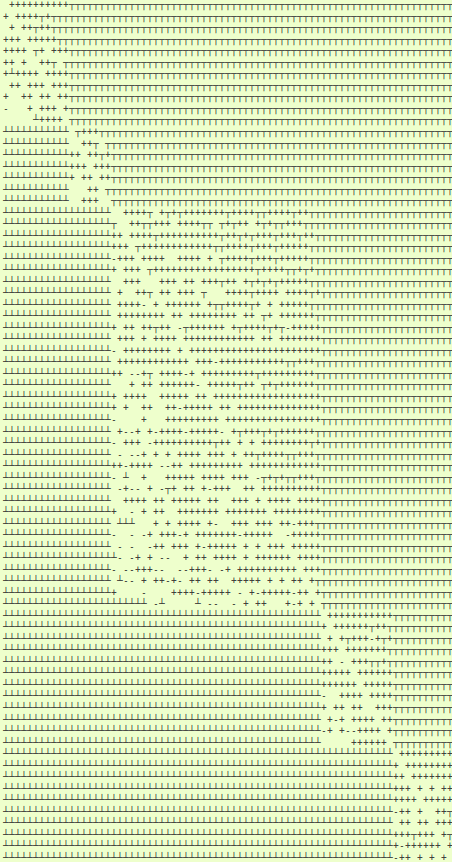
\includegraphics[width=7cm]{Figures/11-1-sparseRelationMap.png}
\caption{Sparse quartiles-sorting decomposed outranking relation (extract). Legend: \emph{outranking} for certain ($\top$); \emph{outranked} for certain ($\bot$); more or less \emph{outranking} ($+$); more or less \emph{outranked} ($-$); \emph{indeterminate}}
\label{fig:11.1}       % Give a unique label
\end{figure}
%\clearpage

With a fill rate of $25\%$, the memory occupation of this sparse outranking digraph \texttt{sg} instance takes now only $769$kB, compared to the $1.7$MB required by a corresponding standard \texttt{BipolarOutrankingDigraph} instance (see List.\vref{list:11.3}).
\begin{lstlisting}
>>> print('%.0fkB' % (total_size(sg)/1024) )
    769kB
\end{lstlisting}

For sparse outranking digraphs, the adjacency table is implemented as a dynamic \texttt{relation()} function instead of a double dictionary.
\begin{lstlisting}[caption={The \texttt{relation()} function of a sparse outranking digraph},label=list:11.4,basicstyle=\ttfamily\scriptsize]
   def relation(self, int x, int y):
       """
       *Parameters*:
           * x (int action key),
           * y (int action key).
       Dynamic construction of the global outranking
       characteristic function *r(x S y)*.
       """
       cdef int Min, Med, Max, rx, ry
       Min = self.valuationdomain['min']
       Med = self.valuationdomain['med']
       Max = self.valuationdomain['max']
       if x == y:
           return Med
       cx = self.actions[x]['component']
       cy = self.actions[y]['component']
       #print(self.components)
       rx = self.components[cx]['rank']
       ry = self.components[cy]['rank']
       if rx == ry:
           try:
               rxpg = self.components[cx]['subGraph'].relation
               return rxpg[x][y]
           except AttributeError:
               componentRanking = self.components[cx]['componentRanking']
               if componentRanking.index(x) < componentRanking.index(x):
                   return Max
               else:
                   return Min
       elif rx > ry:
           return Min
       else:
           return Max
\end{lstlisting}

\section{Quantiles ranking of big performance tableaux}
\label{sec:11.4}

The \texttt{boostedRanking} attribute of the sparse outranking digraph \texttt{sg} contains the global linear ranking of the 100 decision alternatives. This ranking is computed by locally ranking the individual 6 components with the \Copeland rule (see List.~\vref{list:11.3} Lines 12 and 33).
\begin{lstlisting}
>>> sg.boostedRanking
  [22, 53, 3, 34, 56, 62, 24, 44, 50, 93, 41, 63, 29, 58,
   96, 7, 43, 81, 91, 35, 25, 76, 66, 65, 8, 10, 1, 11, 61,
   30, 48, 45, 68, 5, 89, 57, 59, 85, 82, 73, 33, 94, 70,
   97, 20, 92, 71, 90, 95, 21, 28, 2, 36, 87, 40, 98, 46, 55,
   100, 64, 17, 26, 27, 19, 69, 6, 38, 4, 37, 60, 31, 77, 78,
   47, 99, 18, 12, 80, 54, 88, 39, 9, 72, 86, 42, 13, 23, 67,
   52, 15, 32, 49, 51, 74, 16, 14, 75, 79, 83, 84]
\end{lstlisting}

When actually computing linear rankings of the complete set of alternatives, the local outranking relations per component are of no practical usage, and we may furthermore reduce the memory occupation of the resulting digraph by:
\begin{enumerate}[topsep=1pt]
\item refining the ordering of the quantile classes by taking into account how well an alternative is outranking the lower limit of its quantile class, respectively the upper limit of its quantile class is \emph{not} outranking the alternative;
\item dropping the local outranking digraphs and keeping for each component only a locally ranked list of alternatives.
\end{enumerate}

We provide therefore the \texttt{cQuantilesRankingDigraph} class\index{cQuantilesRankingDigraph@\texttt{cQuantilesRankingDigraph} class} from the \texttt{cSparseIntegerOutrankingDigraphs} module.
\begin{lstlisting}[caption={Ranking the sparse integer outranking digraph},label=list:11.5]
>>> from cSparseIntegerOutrankingDigraphs import\
...           cQuantilesRankingDigraph
>>> qr = cQuantilesRankingDigraph(t,4)
>>> qr
 *----- Object instance description --------------*
  Instance class    : cQuantilesRankingDigraph
  Instance name     : cRandomperftab_mp
  Actions           : 100
  Criteria          : 7
  Sorting by        : 4-Tiling
  Ordering strategy : optimal
  Ranking rule      : Copeland
  Components        : 47
  Minimal order     : 1
  Maximal order     : 10
  Average order     : 2.1
  fill rate         : 2.566%
 *----  Constructor run times (in sec.) ----*
  Nbr of threads    : 1
  Total time        : 0.03702
  QuantilesSorting  : 0.01785
  Preordering       : 0.00022
  Decomposing       : 0.01892
  Attributes       : ['runTimes', 'name',
  'actions', 'order', 'dimension', 'sortingParameters',
  'nbrOfCPUs','valuationdomain', 'profiles', 'categories',
  'sorting', 'minimalComponentSize','decomposition',
  'nbrComponents', 'nd', 'components', 'fillRate',
  'maximalComponentSize', 'componentRankingRule', 'boostedRanking']
\end{lstlisting}

With this \emph{optimised} quantile ordering strategy, we obtain now 47 performance equivalence classes (see List.~\vref{list:11.5} Line 13).
\begin{lstlisting}[caption={The ordered components of the sparse outranking digraph},label=list:11.6]
>>> qr.components
    OrderedDict([
    ('c01', {'rank': 1,
	     'lowQtileLimit': ']0.75',
	     'highQtileLimit': '1.00]',
	     'componentRanking': [53]}),
    ('c02', {'rank': 2,
	     'lowQtileLimit': ']0.75',
	     'highQtileLimit': '1.00]',
	     'componentRanking': [3, 23, 63, 50]}),
    ('c03', {'rank': 3,
	     'lowQtileLimit': ']0.75',
	     'highQtileLimit': '1.00]',
	     'componentRanking': [34, 44, 56, 24, 93, 41]}), 
    ...
    ...
    ...
    ('c45', {'rank': 45,
	     'lowQtileLimit': ']0.25',
	     'highQtileLimit': '0.50]',
	     'componentRanking': [49]}),
    ('c46', {'rank': 46,
	     'lowQtileLimit': ']0.25',
	     'highQtileLimit': '0.50]',
	     'componentRanking': [52, 16, 86]}),
    ('c47', {'rank': 47,
	     'lowQtileLimit': ']<',
	     'highQtileLimit': '0.25]',
	     'componentRanking': [79, 83, 84]})])
>>> print('%.0fkB' % (total_size(qr)/1024) )
    208kB
\end{lstlisting}

We observe in Listing~\vref{list:11.6} an even more considerably less voluminous memory occupation 208kB, compared to the 769kB of the \texttt{SparseIntegerOutran\-king\-Digraph} instance.

It is opportune, however, to measure the loss of quality of the resulting \Copeland ranking when working with sparse outranking digraphs.
\begin{lstlisting}[caption={Measuring the loss of quality with respect to the standard outranking digraph},label=list:11.7]
>>> from cIntegerOutrankingDigraphs import\
...                       IntegerBipolarOutrankingDigraph
>>> ig = IntegerBipolarOutrankingDigraph(t)
>>> print('Complete outranking : %+.3f'\
...    % (ig.computeOrderCorrelation(\
...             ig.computeCopelandOrder())['correlation']))
    Complete outranking : +0.747

>>> print('Sparse 4-tiling : %+.3f'\
...     % (ig.computeOrderCorrelation(\
...        list(reversed(sg.boostedRanking)))['correlation']))   
    Sparse 4-tiling          : +0.717

>>> print('Optimzed sparse 4-tiling: %+.3f'\
...  % (ig.computeOrderCorrelation(\
...     list(reversed(qr.boostedRanking)))\
...     ['correlation']))  
    Optimzed sparse 4-tiling: +0.705
\end{lstlisting}

The best ranking correlation with the pairwise outranking situations ($+0.747$) is naturally given when we apply the \Copeland rule to the standard outranking digraph (see List.~\vref{list:10.7} Line 7). When applying the same rule to the sparse 4-tiled outranking digraph, one gets a correlation of $+0.717$ (Line 12), and when applying the \Copeland rule to the optimised sparse 4-tiled digraph, we still obtain a correlation of $+0.705$ (Line 18). These optimistic results actually depend on the number of quantiles we use as well as on the given model of random performance tableau.

In case of \texttt{Random3ObjectivesPerformanceTableau} instances, for instance, we would get in a similar setting an even better standrad outranking correlation of $+0.86$, a sparse 4-tiling correlation of $+0.82$, and an optimised sparse 4-tiling correlation of $+0.81$.

\section{HPC quantiles ranking records}
\label{sec:11.5}

Following from the separability property of the $q$-tiles sorting of each action into a $q$-tiles class, the $q$-sorting algorithm may be safely split into as much threads as are multiple processing cores available for working in parallel (see Prop.~\ref{prop:9.1}). Furthermore, the ranking procedure being local to each diagonal component, these procedures may as well be safely processed in parallel threads on each component restricted outranking digraph.

Using the HPC platform of the University of Luxembourg -- https://hpc-docs.uni.lu/ \citep{UNI-2014}-- the following run times for very big ranking problems could be achieved both on:
\begin{itemize}[topsep=1pt]
\item \emph{Iris -skylake} nodes with 28 cores:\\
  (see \href{https://hpc-docs.uni.lu/systems/iris/}{https://hpc-docs.uni.lu/systems/iris}), and
\item the 3TB -bigmem \emph{Gaia-183} node with 64 cores \\
  (see \href{https://hpc.uni.lu/systems/gaia/}{https://hpc.uni.lu/systems/gaia}),
\end{itemize}
by running the cythonized Python modules in an Intel compiled virtual Python 3.6.5 environment [GCC Intel(R) 17.0.1 –enable-optimizations c++ gcc 6.3 mode] on Debian 8 Linux.

\begin{figure}[ht]
\sidecaption
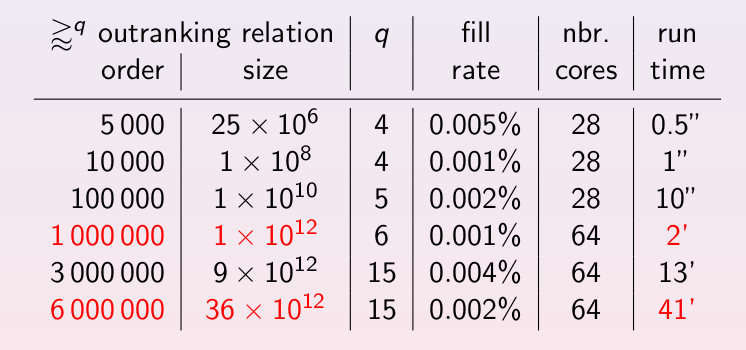
\includegraphics[width=7cm]{Figures/11-2-rankingRecords.png}
\caption{HPC-UL Ranking Performance Records (Spring 2018). On the big memory equipped Gaia-183 node, we were able to rank a million decision alternatives in about 2 minutes. We even could linearly rank up to 6 million decision alternatives in about 40 minutes}
\label{fig:11.2}       % Give a unique label
\end{figure}
  
%%%%%%% The chapter bibliography
%\normallatexbib
%\clearpage
%\phantomsection
%\addcontentsline{toc}{chapter}{Chapter Bibliography}
%\chapter{HPC ranking of big performance tableaux}
\label{sec:11}

\abstract*{ The sparse outranking digraph, introduced inn Chapter~\ref{sec:9} is suitable for tackling the ranking of big multiple criteria performance tableaux with thausands or millions of records. To effectively compute rankings from performance tableaux of these sizes, we propose in this chapter a collection of C-compiled and optimised \Digraph modules that may be run on HPC equipement as available, for instance at the University of Luxembourg.}

\abstract{ The sparse outranking digraph, introduced inn Chapter~\ref{sec:9} is suitable for tackling the ranking of big multiple criteria performance tableaux with thausands or millions of records. To effectively compute rankings from performance tableaux of these sizes, we propose in this chapter a collection of C-compiled and optimised \Digraph modules that may be run on HPC equipement as available, for instance at the University of Luxembourg.}

\section{C-compiled Python modules}
\label{sec:11.1}

The \Digraph collection provides cythonized \footnote{\Cython C-extension for Python, https://cython.org/}, i.e. C-compiled and optimised versions of the main python modules for tackling multiple criteria decision problems facing very large sets of decision alternatives ( $> 10000$ ). Such problems appear usually with a combinatorial organisation of the potential decision alternatives, as is frequently the case in bioinformatics for instance. If HPC facilities with nodes supporting numerous cores ($> 20$) and big RAM ($>$ 50GB) are available, ranking up to several millions of alternatives becomes effectively tractable (see \citep{BIS-2016}).

Four cythonized \Digraph modules, prefixed with the letter \texttt{c} and taking a \texttt{pyx} extension, are provided with their corresponding setup tools in the \texttt{cython} directory of the \Digraph resources, namely:
\begin{itemize}[topsep=1pt]
\item[] \texttt{cRandPerfTabs.pyx},
\item[] \texttt{cIntegerOutrankingDigraphs.pyx},
\item[] \texttt{cIntegerSortingDigraphs.pyx}, and
\item[] \texttt{cSparseIntegerOutrankingDigraphs.pyx}.
\end{itemize}

Their automatic compilation and installation, alongside the standard \Digraph python3 modules, requires the \emph{cython} compiler:

\texttt{...\$ python3 -m pip install cython}

\noindent and a C compiler:

\texttt{...\$ sudo apt install gcc} on Ubuntu, for instance.

These cythonized modules, specifically designed for being run on HPC clusters, require the Unix \emph{forking} start method of subprocesses and therefore, due to forking problems on Mac OS platforms, may only operate safely on Linux platforms (see start methods of the \href{https://docs.python.org/3/library/multiprocessing.html#contexts-and-start-methods}{Python multiprocessing library}).

\section{Big Data performance tableaux}
\label{sec:11.2}

In order to efficiently type the C variables, the \texttt{cRandPerfTabs} module\index{cRandPerfTabs@\texttt{cRandPerfTabs} module} provides the root \texttt{cPerformanceTableau} class\index{cPerformanceTableau@\texttt{cPerformanceTableau} class}, but, with \emph{integer} action keys, \emph{float} performance evaluations, \emph{integer} criteria weights and \emph{float} discrimination thresholds. And, to limit as much as possible memory occupation of class instances, all the usual verbose comments are dropped from the description of the \texttt{actions} and \texttt{criteria} dictionaries. A random instance may be generated with the  \texttt{cRandomPerformanceTableau} class\index{cRandomPerformanceTableau@\texttt{cRandomPerformanceTableau} class}:
\begin{lstlisting}[caption={Big data performance tableau format},label=list:11.1,basicstyle=\ttfamily\scriptsize]
>>> from cRandPerfTabs import cRandomPerformanceTableau
>>> t = cRandomPerformanceTableau(numberOfActions=4,\
...                               numberOfCriteria=2)
>>> t
  *------- PerformanceTableau instance description ------*
    Instance class   : cRandomPerformanceTableau
    Seed             : None
    Instance name    : cRandomperftab
    Actions          : 4
    Criteria         : 2
    Attributes       : ['randomSeed', 'name', 'actions',
                        'criteria', 'evaluation', 'weightPreorder']
>>> t.actions
   OrderedDict([(1, {'name': '#1'}), (2, {'name': '#2'}),
		(3, {'name': '#3'}), (4, {'name': '#4'})])
>>> t.criteria
   OrderedDict([
   ('g1', {'name': 'RandomPerformanceTableau() instance',
	       'thresholds': {'ind': (10.0, 0.0),
			       'pref': (20.0, 0.0),
			       'veto': (80.0, 0.0)},
	       'scale': (0.0, 100.0),
	       'weight': 1,
	       'preferenceDirection': 'max'}),
   ('g2', {'name': 'RandomPerformanceTableau() instance',
	       'thresholds': {'ind': (10.0, 0.0),
			       'pref': (20.0, 0.0),
			       'veto': (80.0, 0.0)},
	       'scale': (0.0, 100.0),
	       'weight': 1,
	       'preferenceDirection': 'max'})])
>>> t.evaluation
  {'g1': {1: 35.17, 2: 56.4, 3: 1.94, 4: 5.51},
   'g2': {1: 95.12, 2: 90.54, 3: 51.84, 4: 15.42}}
>>> t.showPerformanceTableau()
	Criteria |  'g1'    'g2'   
	Actions  |    1       1    
	---------|---------------
	   '#1'  |  91.18   90.42  
	   '#2'  |  66.82   41.31  
	   '#3'  |  35.76   28.86  
	   '#4'  |   7.78   37.64  
\end{lstlisting}

Several methods for converting from the Big Data model to the standard model and vice versa are provided by the \texttt{cPerformanceTableau} class.\index{convert2Standard@\texttt{convert2Standard()}}\index{convertWeight2Decimal@\texttt{convertWeight2Decimal()}}\index{convertEvaluation2Decimal@\texttt{convertEvaluation2Decimal()}}
\begin{lstlisting}   
>>> t1 = t.convert2Standard()
>>> t1.convertWeight2Decimal()
>>> t1.convertEvaluation2Decimal()
>>> t1
  *------- PerformanceTableau instance description ------*
   Instance class   : PerformanceTableau
   Seed             : None
   Instance name    : std_cRandomperftab
   Actions          : 4
   Criteria         : 2
   Attributes       : ['name', 'actions', 'criteria',
                       'weightPreorder', 'evaluation',
                       'randomSeed']
\end{lstlisting}

\section{C-implemented integer-valued outranking digraphs}
\label{sec:11.3}

The C compiled version of the \texttt{BipolarOutrankingDigraph} class takes integer $r$-characteristic values.\index{cIntegerOutrankingDigraphs@\texttt{cIntegerOutrankingDigraphs} module}\index{IntegerBipolarOutrankingDigraph@\texttt{IntegerBipolarOutrankingDigraph} class}
\begin{lstlisting}[caption={Constructing big bipolar-valued outranking digraphs},label=list:11.2]
>>> from cRandPerfTabs import cRandomPerformanceTableau
>>> t = cRandomPerformanceTableau(numberOfActions=1000,\
...                               numberOfCriteria=2,seed=100)
>>> from cIntegerOutrankingDigraphs import\
...                 IntegerBipolarOutrankingDigraph
>>> g = IntegerBipolarOutrankingDigraph(t,\
...                 Threading=True, nbrCores=4)
>>> g
  *------- Object instance description ------*
   Instance class   : IntegerBipolarOutrankingDigraph
   Instance name    : rel_cRandomperftab
   Actions          : 1000
   Criteria         : 2
   Size             : 460795
   Determinateness  : 55.975
   Valuation domain : {'min': -2, 'med': 0, 'max': 2,
                       'hasIntegerValuation': True}
   ----  Constructor run times (in sec.) ----
   Total time       : 4.10093
   Data input       : 0.00955
   Compute relation : 3.33437
   Gamma sets       : 0.75699
   Size             : 465024
   Determinateness  : 56.877
   Attributes       : ['name', 'actions', 'criteria',
                       'totalWeight', 'valuationdomain',
                       'methodData', 'evaluation',
                       'order', 'runTimes', 'nbrThreads',
                       'relation', 'gamma', 'notGamma']
\end{lstlisting}

On a classical intel-i7 equipped PC with four single threaded cores, the \texttt{Inte\-ger\-BipolarOutrankingDigraph} class constructor takes about four seconds for computing a \emph{million} pairwise outranking characteristic values (see List.~\vref{list:11.2}). In a similar setting, the standard \texttt{BipolarOutranking\-Digraph} constructor operates more than two times slower.
\begin{lstlisting}
>>> from outrankingDigraphs import BipolarOutrankingDigraph
>>> t1 = t.convert2Standard()
>>> g1 = BipolarOutrankingDigraph(t1,\
...                Threading=True,nbrCores=4)
>>> g1
  *------- Object instance description ------*
    Instance class       : BipolarOutrankingDigraph
    Instance name        : rel_std_cRandomperftab
    Actions              : 1000
    Criteria             : 2
    Size                 : 460795
    Determinateness (%)  : 77.99
    Valuation domain     : [-1.00;1.00]
    Attributes           : ['name','actions','valuationdomain',
                            'criteria','methodData','evaluation',
                            'NA','order','runTimes','nbrThreads',
                            'relation','gamma','notGamma']
    ----  Constructor run times (in sec.) ----
    Total time           : 14.92166
    Data input           : 0.01506
    Compute relation     : 13.51562
    Gamma sets           : 1.39096
    Threads              : 4
\end{lstlisting}

By far, most of the run time is in each case needed for computing the individual pairwise outranking characteristic values: $4.10$ sec. versus $14.92$ sec. Notice also below the memory occupations --about 108MB for \texttt{g} and 216MB for \texttt{g1}-- of both outranking digraph instances.\index{digraphsTools@\texttt{digraphsTools} module}\index{total-size@\texttt{total\_size()}}
\begin{lstlisting}
>>> from digraphsTools import total_size
>>> total_size(g)
    107503580
>>> total_size(g1)
    211519995
>>> total_size(g1.relation)/total_size(g1)
    0.67
>>> total_size(g1.gamma)/total_size(g1)
    0.23
\end{lstlisting}

The standard \texttt{Decimal} valued \texttt{BipolarOutrankingDigraph} instance \texttt{g1} thus nearly doubles the memory occupation of the corresponding \texttt{IntegerBipo\-larOutrankingDigraph} \texttt{g} instance (see Line 3 and 5 above). $90\%$ of this memory occupation is due to the \texttt{g1.relation} ($67\%$) and the \texttt{g1.gamma} ($23\%$) dictionaries. And these ratios quadratically grow with the digraph order. To limit the object sizes for really big outranking digraphs, we need to abandon the complete implementation of adjacency tables and gamma functions.

\section{The sparse implementation of big outranking digraphs}
\label{sec:11.4}

The idea is to first decompose the complete outranking relation into an ordered collection of equivalent quantile performance classes. Let us consider for this illustration a random performance tableau with 100 decision alternatives evaluated on 7 criteria.
\begin{lstlisting}
>>> from cRandPerfTabs import cRandomPerformanceTableau
>>> t = cRandomPerformanceTableau(numberOfActions=100,\
...                       numberOfCriteria=7,seed=100)
\end{lstlisting}

The \texttt{cSparseIntegerOutrankingDigraphs} module\index{cSparseIntegerOutrankingDigraphs@\texttt{cSparseIntegerOutrankingDigraphs} module} provides the \texttt{Spar\-seIntegerOutrankingDigraph} class\index{SparseIntegerOutrankingDigraph@\texttt{SparseIntegerOutrankingDigraph} class} for sorting the $100$ decision alternatives into overlapping quartile classes and rank all $100$ with respect to the average quantile limits.
\begin{lstlisting}[caption={Constructing the sparse integer outranking digraph},label=list:11.3]
>>> from cSparseIntegerOutrankingDigraphs import\
...                    SparseIntegerOutrankingDigraph
>>> sg = SparseIntegerOutrankingDigraph(t,quantiles=4)
>>> sg
  *----- Object instance description --------------*
   Instance class    : SparseIntegerOutrankingDigraph
   Instance name     : cRandomperftab_mp
   Actions           : 100
   Criteria          : 7
   Sorting by        : 4-Tiling
   Ordering strategy : average
   Ranking rule      : Copeland
   Components        : 6
   Minimal order     : 1
   Maximal order     : 35
   Average order     : 16.7
   fill rate         : 24.970%
  *----  Constructor run times (in sec.) ----
   Nbr of threads    : 1
   Total time        : 0.08212
   QuantilesSorting  : 0.01481
   Preordering       : 0.00022
   Decomposing       : 0.06707
   Ordering          : 0.00000
   Attributes       : ['runTimes', 'name', 'actions',
       'criteria', 'evaluation', 'order', 'dimension',
       'sortingParameters', 'nbrOfCPUs',
       'valuationdomain', 'profiles', 'categories',
       'sorting', 'minimalComponentSize',
       'decomposition', 'nbrComponents', 'nd',
       'components', 'fillRate',
       'maximalComponentSize', 'componentRankingRule',
       'boostedRanking']
\end{lstlisting}

We obtain in this example here a decomposition into 6 linearly ordered components with a maximal component size of 35 for component \texttt{c3}.

\begin{lstlisting}
>>> sg.showDecomposition()
 *--- quantiles decomposition in decreasing order---*
  c1. ]0.75-1.00] : [3,22,24,34,41,44,50,53,56,62,93]
  c2. ]0.50-1.00] : [7,29,43,58,63,81,96]
  c3. ]0.50-0.75] : [1,2,5,8,10,11,20,21,25,28,30,33,
                     35,36,45,48,57,59,61,65,66,68,70,
                     71,73,76,82,85,89,90,91,92,94,95,97]
  c4. ]0.25-0.75] : [17,19,26,27,40,46,55,64,69,87,98,100]
  c5. ]0.25-0.50] : [4,6,9,12,13,14,15,16,18,23,31,32,
                     37,38,39,42,47,49,51,52,54,60,67,72,
                     74,75,77,78,80,86,88,99]
  c6. ]<-0.25]    : [79,83,84]
\end{lstlisting}

A restricted outranking relation is stored for each component with more than one alternative. The showRelationMap() prints out below the relation map of the sparse digraph \texttt{sg} for the 75 first-ranked alternatives. (see Fig.~\vref{fig:11.1}):
\begin{lstlisting}
>>> sg.showRelationMap(toIndex=75)
\end{lstlisting}  
\begin{figure}[ht]
\sidecaption[t]
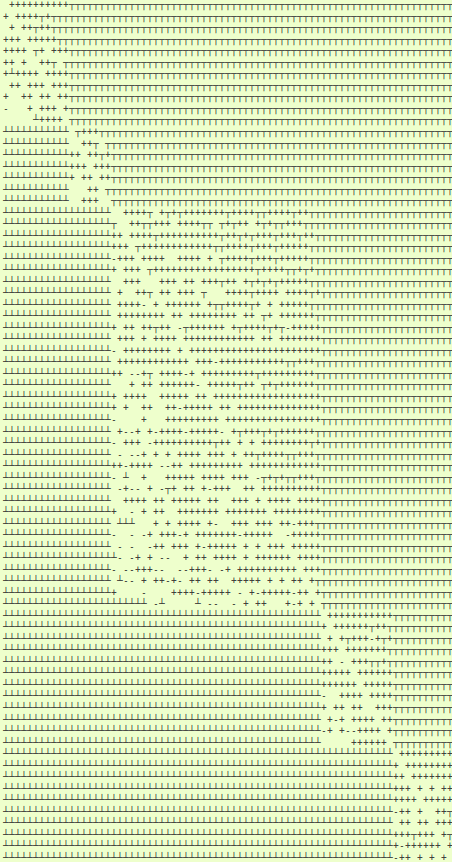
\includegraphics[width=7cm]{Figures/11-1-sparseRelationMap.png}
\caption{Sparse quartiles-sorting decomposed outranking relation (extract). Legend: \emph{outranking} for certain ($\top$); \emph{outranked} for certain ($\bot$); more or less \emph{outranking} ($+$); more or less \emph{outranked} ($-$); \emph{indeterminate}}
\label{fig:11.1}       % Give a unique label
\end{figure}
%\clearpage

With a fill rate of $25\%$, the memory occupation of this sparse outranking digraph \texttt{sg} instance takes now only $769$kB, compared to the $1.7$MB required by a corresponding standard \texttt{BipolarOutrankingDigraph} instance (see List.\vref{list:11.3}).
\begin{lstlisting}
>>> print('%.0fkB' % (total_size(sg)/1024) )
    769kB
\end{lstlisting}

For sparse outranking digraphs, the adjacency table is implemented as a dynamic \texttt{relation()} function instead of a double dictionary.
\begin{lstlisting}[caption={The \texttt{relation()} function of a sparse outranking digraph},label=list:11.4,basicstyle=\ttfamily\scriptsize]
   def relation(self, int x, int y):
       """
       *Parameters*:
           * x (int action key),
           * y (int action key).
       Dynamic construction of the global outranking
       characteristic function *r(x S y)*.
       """
       cdef int Min, Med, Max, rx, ry
       Min = self.valuationdomain['min']
       Med = self.valuationdomain['med']
       Max = self.valuationdomain['max']
       if x == y:
           return Med
       cx = self.actions[x]['component']
       cy = self.actions[y]['component']
       #print(self.components)
       rx = self.components[cx]['rank']
       ry = self.components[cy]['rank']
       if rx == ry:
           try:
               rxpg = self.components[cx]['subGraph'].relation
               return rxpg[x][y]
           except AttributeError:
               componentRanking = self.components[cx]['componentRanking']
               if componentRanking.index(x) < componentRanking.index(x):
                   return Max
               else:
                   return Min
       elif rx > ry:
           return Min
       else:
           return Max
\end{lstlisting}

\section{Quantiles ranking of big performance tableaux}
\label{sec:11.4}

The \texttt{boostedRanking} attribute of the sparse outranking digraph \texttt{sg} contains the global linear ranking of the 100 decision alternatives. This ranking is computed by locally ranking the individual 6 components with the \Copeland rule (see List.~\vref{list:11.3} Lines 12 and 33).
\begin{lstlisting}
>>> sg.boostedRanking
  [22, 53, 3, 34, 56, 62, 24, 44, 50, 93, 41, 63, 29, 58,
   96, 7, 43, 81, 91, 35, 25, 76, 66, 65, 8, 10, 1, 11, 61,
   30, 48, 45, 68, 5, 89, 57, 59, 85, 82, 73, 33, 94, 70,
   97, 20, 92, 71, 90, 95, 21, 28, 2, 36, 87, 40, 98, 46, 55,
   100, 64, 17, 26, 27, 19, 69, 6, 38, 4, 37, 60, 31, 77, 78,
   47, 99, 18, 12, 80, 54, 88, 39, 9, 72, 86, 42, 13, 23, 67,
   52, 15, 32, 49, 51, 74, 16, 14, 75, 79, 83, 84]
\end{lstlisting}

When actually computing linear rankings of the complete set of alternatives, the local outranking relations per component are of no practical usage, and we may furthermore reduce the memory occupation of the resulting digraph by:
\begin{enumerate}[topsep=1pt]
\item refining the ordering of the quantile classes by taking into account how well an alternative is outranking the lower limit of its quantile class, respectively the upper limit of its quantile class is \emph{not} outranking the alternative;
\item dropping the local outranking digraphs and keeping for each component only a locally ranked list of alternatives.
\end{enumerate}

We provide therefore the \texttt{cQuantilesRankingDigraph} class\index{cQuantilesRankingDigraph@\texttt{cQuantilesRankingDigraph} class} from the \texttt{cSparseIntegerOutrankingDigraphs} module.
\begin{lstlisting}[caption={Ranking the sparse integer outranking digraph},label=list:11.5]
>>> from cSparseIntegerOutrankingDigraphs import\
...           cQuantilesRankingDigraph
>>> qr = cQuantilesRankingDigraph(t,4)
>>> qr
 *----- Object instance description --------------*
  Instance class    : cQuantilesRankingDigraph
  Instance name     : cRandomperftab_mp
  Actions           : 100
  Criteria          : 7
  Sorting by        : 4-Tiling
  Ordering strategy : optimal
  Ranking rule      : Copeland
  Components        : 47
  Minimal order     : 1
  Maximal order     : 10
  Average order     : 2.1
  fill rate         : 2.566%
 *----  Constructor run times (in sec.) ----*
  Nbr of threads    : 1
  Total time        : 0.03702
  QuantilesSorting  : 0.01785
  Preordering       : 0.00022
  Decomposing       : 0.01892
  Attributes       : ['runTimes', 'name',
  'actions', 'order', 'dimension', 'sortingParameters',
  'nbrOfCPUs','valuationdomain', 'profiles', 'categories',
  'sorting', 'minimalComponentSize','decomposition',
  'nbrComponents', 'nd', 'components', 'fillRate',
  'maximalComponentSize', 'componentRankingRule', 'boostedRanking']
\end{lstlisting}

With this \emph{optimised} quantile ordering strategy, we obtain now 47 performance equivalence classes (see List.~\vref{list:11.5} Line 13).
\begin{lstlisting}[caption={The ordered components of the sparse outranking digraph},label=list:11.6]
>>> qr.components
    OrderedDict([
    ('c01', {'rank': 1,
	     'lowQtileLimit': ']0.75',
	     'highQtileLimit': '1.00]',
	     'componentRanking': [53]}),
    ('c02', {'rank': 2,
	     'lowQtileLimit': ']0.75',
	     'highQtileLimit': '1.00]',
	     'componentRanking': [3, 23, 63, 50]}),
    ('c03', {'rank': 3,
	     'lowQtileLimit': ']0.75',
	     'highQtileLimit': '1.00]',
	     'componentRanking': [34, 44, 56, 24, 93, 41]}), 
    ...
    ...
    ...
    ('c45', {'rank': 45,
	     'lowQtileLimit': ']0.25',
	     'highQtileLimit': '0.50]',
	     'componentRanking': [49]}),
    ('c46', {'rank': 46,
	     'lowQtileLimit': ']0.25',
	     'highQtileLimit': '0.50]',
	     'componentRanking': [52, 16, 86]}),
    ('c47', {'rank': 47,
	     'lowQtileLimit': ']<',
	     'highQtileLimit': '0.25]',
	     'componentRanking': [79, 83, 84]})])
>>> print('%.0fkB' % (total_size(qr)/1024) )
    208kB
\end{lstlisting}

We observe in Listing~\vref{list:11.6} an even more considerably less voluminous memory occupation 208kB, compared to the 769kB of the \texttt{SparseIntegerOutran\-king\-Digraph} instance.

It is opportune, however, to measure the loss of quality of the resulting \Copeland ranking when working with sparse outranking digraphs.
\begin{lstlisting}[caption={Measuring the loss of quality with respect to the standard outranking digraph},label=list:11.7]
>>> from cIntegerOutrankingDigraphs import\
...                       IntegerBipolarOutrankingDigraph
>>> ig = IntegerBipolarOutrankingDigraph(t)
>>> print('Complete outranking : %+.3f'\
...    % (ig.computeOrderCorrelation(\
...             ig.computeCopelandOrder())['correlation']))
    Complete outranking : +0.747

>>> print('Sparse 4-tiling : %+.3f'\
...     % (ig.computeOrderCorrelation(\
...        list(reversed(sg.boostedRanking)))['correlation']))   
    Sparse 4-tiling          : +0.717

>>> print('Optimzed sparse 4-tiling: %+.3f'\
...  % (ig.computeOrderCorrelation(\
...     list(reversed(qr.boostedRanking)))\
...     ['correlation']))  
    Optimzed sparse 4-tiling: +0.705
\end{lstlisting}

The best ranking correlation with the pairwise outranking situations ($+0.747$) is naturally given when we apply the \Copeland rule to the standard outranking digraph (see List.~\vref{list:10.7} Line 7). When applying the same rule to the sparse 4-tiled outranking digraph, one gets a correlation of $+0.717$ (Line 12), and when applying the \Copeland rule to the optimised sparse 4-tiled digraph, we still obtain a correlation of $+0.705$ (Line 18). These optimistic results actually depend on the number of quantiles we use as well as on the given model of random performance tableau.

In case of \texttt{Random3ObjectivesPerformanceTableau} instances, for instance, we would get in a similar setting an even better standrad outranking correlation of $+0.86$, a sparse 4-tiling correlation of $+0.82$, and an optimised sparse 4-tiling correlation of $+0.81$.

\section{HPC quantiles ranking records}
\label{sec:11.5}

Following from the separability property of the $q$-tiles sorting of each action into a $q$-tiles class, the $q$-sorting algorithm may be safely split into as much threads as are multiple processing cores available for working in parallel (see Prop.~\ref{prop:9.1}). Furthermore, the ranking procedure being local to each diagonal component, these procedures may as well be safely processed in parallel threads on each component restricted outranking digraph.

Using the HPC platform of the University of Luxembourg -- https://hpc-docs.uni.lu/ \citep{UNI-2014}-- the following run times for very big ranking problems could be achieved both on:
\begin{itemize}[topsep=1pt]
\item \emph{Iris -skylake} nodes with 28 cores:\\
  (see \href{https://hpc-docs.uni.lu/systems/iris/}{https://hpc-docs.uni.lu/systems/iris}), and
\item the 3TB -bigmem \emph{Gaia-183} node with 64 cores \\
  (see \href{https://hpc.uni.lu/systems/gaia/}{https://hpc.uni.lu/systems/gaia}),
\end{itemize}
by running the cythonized Python modules in an Intel compiled virtual Python 3.6.5 environment [GCC Intel(R) 17.0.1 –enable-optimizations c++ gcc 6.3 mode] on Debian 8 Linux.

\begin{figure}[ht]
\sidecaption
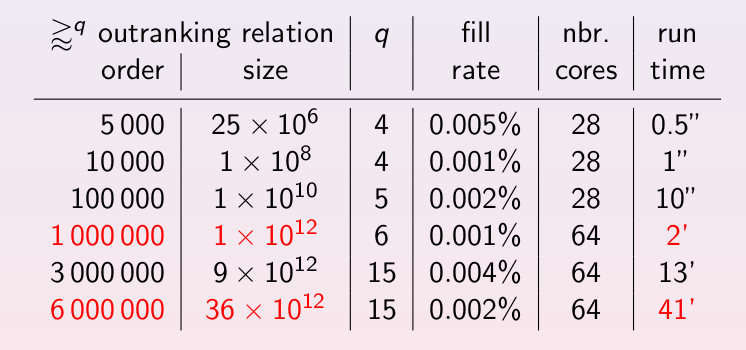
\includegraphics[width=7cm]{Figures/11-2-rankingRecords.png}
\caption{HPC-UL Ranking Performance Records (Spring 2018). On the big memory equipped Gaia-183 node, we were able to rank a million decision alternatives in about 2 minutes. We even could linearly rank up to 6 million decision alternatives in about 40 minutes}
\label{fig:11.2}       % Give a unique label
\end{figure}
  
%%%%%%% The chapter bibliography
%\normallatexbib
%\clearpage
%\phantomsection
%\addcontentsline{toc}{chapter}{Chapter Bibliography}
%\chapter{HPC ranking of big performance tableaux}
\label{sec:11}

\abstract*{ The sparse outranking digraph, introduced inn Chapter~\ref{sec:9} is suitable for tackling the ranking of big multiple criteria performance tableaux with thausands or millions of records. To effectively compute rankings from performance tableaux of these sizes, we propose in this chapter a collection of C-compiled and optimised \Digraph modules that may be run on HPC equipement as available, for instance at the University of Luxembourg.}

\abstract{ The sparse outranking digraph, introduced inn Chapter~\ref{sec:9} is suitable for tackling the ranking of big multiple criteria performance tableaux with thausands or millions of records. To effectively compute rankings from performance tableaux of these sizes, we propose in this chapter a collection of C-compiled and optimised \Digraph modules that may be run on HPC equipement as available, for instance at the University of Luxembourg.}

\section{C-compiled Python modules}
\label{sec:11.1}

The \Digraph collection provides cythonized \footnote{\Cython C-extension for Python, https://cython.org/}, i.e. C-compiled and optimised versions of the main python modules for tackling multiple criteria decision problems facing very large sets of decision alternatives ( $> 10000$ ). Such problems appear usually with a combinatorial organisation of the potential decision alternatives, as is frequently the case in bioinformatics for instance. If HPC facilities with nodes supporting numerous cores ($> 20$) and big RAM ($>$ 50GB) are available, ranking up to several millions of alternatives becomes effectively tractable (see \citep{BIS-2016}).

Four cythonized \Digraph modules, prefixed with the letter \texttt{c} and taking a \texttt{pyx} extension, are provided with their corresponding setup tools in the \texttt{cython} directory of the \Digraph resources, namely:
\begin{itemize}[topsep=1pt]
\item[] \texttt{cRandPerfTabs.pyx},
\item[] \texttt{cIntegerOutrankingDigraphs.pyx},
\item[] \texttt{cIntegerSortingDigraphs.pyx}, and
\item[] \texttt{cSparseIntegerOutrankingDigraphs.pyx}.
\end{itemize}

Their automatic compilation and installation, alongside the standard \Digraph python3 modules, requires the \emph{cython} compiler:

\texttt{...\$ python3 -m pip install cython}

\noindent and a C compiler:

\texttt{...\$ sudo apt install gcc} on Ubuntu, for instance.

These cythonized modules, specifically designed for being run on HPC clusters, require the Unix \emph{forking} start method of subprocesses and therefore, due to forking problems on Mac OS platforms, may only operate safely on Linux platforms (see start methods of the \href{https://docs.python.org/3/library/multiprocessing.html#contexts-and-start-methods}{Python multiprocessing library}).

\section{Big Data performance tableaux}
\label{sec:11.2}

In order to efficiently type the C variables, the \texttt{cRandPerfTabs} module\index{cRandPerfTabs@\texttt{cRandPerfTabs} module} provides the root \texttt{cPerformanceTableau} class\index{cPerformanceTableau@\texttt{cPerformanceTableau} class}, but, with \emph{integer} action keys, \emph{float} performance evaluations, \emph{integer} criteria weights and \emph{float} discrimination thresholds. And, to limit as much as possible memory occupation of class instances, all the usual verbose comments are dropped from the description of the \texttt{actions} and \texttt{criteria} dictionaries. A random instance may be generated with the  \texttt{cRandomPerformanceTableau} class\index{cRandomPerformanceTableau@\texttt{cRandomPerformanceTableau} class}:
\begin{lstlisting}[caption={Big data performance tableau format},label=list:11.1,basicstyle=\ttfamily\scriptsize]
>>> from cRandPerfTabs import cRandomPerformanceTableau
>>> t = cRandomPerformanceTableau(numberOfActions=4,\
...                               numberOfCriteria=2)
>>> t
  *------- PerformanceTableau instance description ------*
    Instance class   : cRandomPerformanceTableau
    Seed             : None
    Instance name    : cRandomperftab
    Actions          : 4
    Criteria         : 2
    Attributes       : ['randomSeed', 'name', 'actions',
                        'criteria', 'evaluation', 'weightPreorder']
>>> t.actions
   OrderedDict([(1, {'name': '#1'}), (2, {'name': '#2'}),
		(3, {'name': '#3'}), (4, {'name': '#4'})])
>>> t.criteria
   OrderedDict([
   ('g1', {'name': 'RandomPerformanceTableau() instance',
	       'thresholds': {'ind': (10.0, 0.0),
			       'pref': (20.0, 0.0),
			       'veto': (80.0, 0.0)},
	       'scale': (0.0, 100.0),
	       'weight': 1,
	       'preferenceDirection': 'max'}),
   ('g2', {'name': 'RandomPerformanceTableau() instance',
	       'thresholds': {'ind': (10.0, 0.0),
			       'pref': (20.0, 0.0),
			       'veto': (80.0, 0.0)},
	       'scale': (0.0, 100.0),
	       'weight': 1,
	       'preferenceDirection': 'max'})])
>>> t.evaluation
  {'g1': {1: 35.17, 2: 56.4, 3: 1.94, 4: 5.51},
   'g2': {1: 95.12, 2: 90.54, 3: 51.84, 4: 15.42}}
>>> t.showPerformanceTableau()
	Criteria |  'g1'    'g2'   
	Actions  |    1       1    
	---------|---------------
	   '#1'  |  91.18   90.42  
	   '#2'  |  66.82   41.31  
	   '#3'  |  35.76   28.86  
	   '#4'  |   7.78   37.64  
\end{lstlisting}

Several methods for converting from the Big Data model to the standard model and vice versa are provided by the \texttt{cPerformanceTableau} class.\index{convert2Standard@\texttt{convert2Standard()}}\index{convertWeight2Decimal@\texttt{convertWeight2Decimal()}}\index{convertEvaluation2Decimal@\texttt{convertEvaluation2Decimal()}}
\begin{lstlisting}   
>>> t1 = t.convert2Standard()
>>> t1.convertWeight2Decimal()
>>> t1.convertEvaluation2Decimal()
>>> t1
  *------- PerformanceTableau instance description ------*
   Instance class   : PerformanceTableau
   Seed             : None
   Instance name    : std_cRandomperftab
   Actions          : 4
   Criteria         : 2
   Attributes       : ['name', 'actions', 'criteria',
                       'weightPreorder', 'evaluation',
                       'randomSeed']
\end{lstlisting}

\section{C-implemented integer-valued outranking digraphs}
\label{sec:11.3}

The C compiled version of the \texttt{BipolarOutrankingDigraph} class takes integer $r$-characteristic values.\index{cIntegerOutrankingDigraphs@\texttt{cIntegerOutrankingDigraphs} module}\index{IntegerBipolarOutrankingDigraph@\texttt{IntegerBipolarOutrankingDigraph} class}
\begin{lstlisting}[caption={Constructing big bipolar-valued outranking digraphs},label=list:11.2]
>>> from cRandPerfTabs import cRandomPerformanceTableau
>>> t = cRandomPerformanceTableau(numberOfActions=1000,\
...                               numberOfCriteria=2,seed=100)
>>> from cIntegerOutrankingDigraphs import\
...                 IntegerBipolarOutrankingDigraph
>>> g = IntegerBipolarOutrankingDigraph(t,\
...                 Threading=True, nbrCores=4)
>>> g
  *------- Object instance description ------*
   Instance class   : IntegerBipolarOutrankingDigraph
   Instance name    : rel_cRandomperftab
   Actions          : 1000
   Criteria         : 2
   Size             : 460795
   Determinateness  : 55.975
   Valuation domain : {'min': -2, 'med': 0, 'max': 2,
                       'hasIntegerValuation': True}
   ----  Constructor run times (in sec.) ----
   Total time       : 4.10093
   Data input       : 0.00955
   Compute relation : 3.33437
   Gamma sets       : 0.75699
   Size             : 465024
   Determinateness  : 56.877
   Attributes       : ['name', 'actions', 'criteria',
                       'totalWeight', 'valuationdomain',
                       'methodData', 'evaluation',
                       'order', 'runTimes', 'nbrThreads',
                       'relation', 'gamma', 'notGamma']
\end{lstlisting}

On a classical intel-i7 equipped PC with four single threaded cores, the \texttt{Inte\-ger\-BipolarOutrankingDigraph} class constructor takes about four seconds for computing a \emph{million} pairwise outranking characteristic values (see List.~\vref{list:11.2}). In a similar setting, the standard \texttt{BipolarOutranking\-Digraph} constructor operates more than two times slower.
\begin{lstlisting}
>>> from outrankingDigraphs import BipolarOutrankingDigraph
>>> t1 = t.convert2Standard()
>>> g1 = BipolarOutrankingDigraph(t1,\
...                Threading=True,nbrCores=4)
>>> g1
  *------- Object instance description ------*
    Instance class       : BipolarOutrankingDigraph
    Instance name        : rel_std_cRandomperftab
    Actions              : 1000
    Criteria             : 2
    Size                 : 460795
    Determinateness (%)  : 77.99
    Valuation domain     : [-1.00;1.00]
    Attributes           : ['name','actions','valuationdomain',
                            'criteria','methodData','evaluation',
                            'NA','order','runTimes','nbrThreads',
                            'relation','gamma','notGamma']
    ----  Constructor run times (in sec.) ----
    Total time           : 14.92166
    Data input           : 0.01506
    Compute relation     : 13.51562
    Gamma sets           : 1.39096
    Threads              : 4
\end{lstlisting}

By far, most of the run time is in each case needed for computing the individual pairwise outranking characteristic values: $4.10$ sec. versus $14.92$ sec. Notice also below the memory occupations --about 108MB for \texttt{g} and 216MB for \texttt{g1}-- of both outranking digraph instances.\index{digraphsTools@\texttt{digraphsTools} module}\index{total-size@\texttt{total\_size()}}
\begin{lstlisting}
>>> from digraphsTools import total_size
>>> total_size(g)
    107503580
>>> total_size(g1)
    211519995
>>> total_size(g1.relation)/total_size(g1)
    0.67
>>> total_size(g1.gamma)/total_size(g1)
    0.23
\end{lstlisting}

The standard \texttt{Decimal} valued \texttt{BipolarOutrankingDigraph} instance \texttt{g1} thus nearly doubles the memory occupation of the corresponding \texttt{IntegerBipo\-larOutrankingDigraph} \texttt{g} instance (see Line 3 and 5 above). $90\%$ of this memory occupation is due to the \texttt{g1.relation} ($67\%$) and the \texttt{g1.gamma} ($23\%$) dictionaries. And these ratios quadratically grow with the digraph order. To limit the object sizes for really big outranking digraphs, we need to abandon the complete implementation of adjacency tables and gamma functions.

\section{The sparse implementation of big outranking digraphs}
\label{sec:11.4}

The idea is to first decompose the complete outranking relation into an ordered collection of equivalent quantile performance classes. Let us consider for this illustration a random performance tableau with 100 decision alternatives evaluated on 7 criteria.
\begin{lstlisting}
>>> from cRandPerfTabs import cRandomPerformanceTableau
>>> t = cRandomPerformanceTableau(numberOfActions=100,\
...                       numberOfCriteria=7,seed=100)
\end{lstlisting}

The \texttt{cSparseIntegerOutrankingDigraphs} module\index{cSparseIntegerOutrankingDigraphs@\texttt{cSparseIntegerOutrankingDigraphs} module} provides the \texttt{Spar\-seIntegerOutrankingDigraph} class\index{SparseIntegerOutrankingDigraph@\texttt{SparseIntegerOutrankingDigraph} class} for sorting the $100$ decision alternatives into overlapping quartile classes and rank all $100$ with respect to the average quantile limits.
\begin{lstlisting}[caption={Constructing the sparse integer outranking digraph},label=list:11.3]
>>> from cSparseIntegerOutrankingDigraphs import\
...                    SparseIntegerOutrankingDigraph
>>> sg = SparseIntegerOutrankingDigraph(t,quantiles=4)
>>> sg
  *----- Object instance description --------------*
   Instance class    : SparseIntegerOutrankingDigraph
   Instance name     : cRandomperftab_mp
   Actions           : 100
   Criteria          : 7
   Sorting by        : 4-Tiling
   Ordering strategy : average
   Ranking rule      : Copeland
   Components        : 6
   Minimal order     : 1
   Maximal order     : 35
   Average order     : 16.7
   fill rate         : 24.970%
  *----  Constructor run times (in sec.) ----
   Nbr of threads    : 1
   Total time        : 0.08212
   QuantilesSorting  : 0.01481
   Preordering       : 0.00022
   Decomposing       : 0.06707
   Ordering          : 0.00000
   Attributes       : ['runTimes', 'name', 'actions',
       'criteria', 'evaluation', 'order', 'dimension',
       'sortingParameters', 'nbrOfCPUs',
       'valuationdomain', 'profiles', 'categories',
       'sorting', 'minimalComponentSize',
       'decomposition', 'nbrComponents', 'nd',
       'components', 'fillRate',
       'maximalComponentSize', 'componentRankingRule',
       'boostedRanking']
\end{lstlisting}

We obtain in this example here a decomposition into 6 linearly ordered components with a maximal component size of 35 for component \texttt{c3}.

\begin{lstlisting}
>>> sg.showDecomposition()
 *--- quantiles decomposition in decreasing order---*
  c1. ]0.75-1.00] : [3,22,24,34,41,44,50,53,56,62,93]
  c2. ]0.50-1.00] : [7,29,43,58,63,81,96]
  c3. ]0.50-0.75] : [1,2,5,8,10,11,20,21,25,28,30,33,
                     35,36,45,48,57,59,61,65,66,68,70,
                     71,73,76,82,85,89,90,91,92,94,95,97]
  c4. ]0.25-0.75] : [17,19,26,27,40,46,55,64,69,87,98,100]
  c5. ]0.25-0.50] : [4,6,9,12,13,14,15,16,18,23,31,32,
                     37,38,39,42,47,49,51,52,54,60,67,72,
                     74,75,77,78,80,86,88,99]
  c6. ]<-0.25]    : [79,83,84]
\end{lstlisting}

A restricted outranking relation is stored for each component with more than one alternative. The showRelationMap() prints out below the relation map of the sparse digraph \texttt{sg} for the 75 first-ranked alternatives. (see Fig.~\vref{fig:11.1}):
\begin{lstlisting}
>>> sg.showRelationMap(toIndex=75)
\end{lstlisting}  
\begin{figure}[ht]
\sidecaption[t]
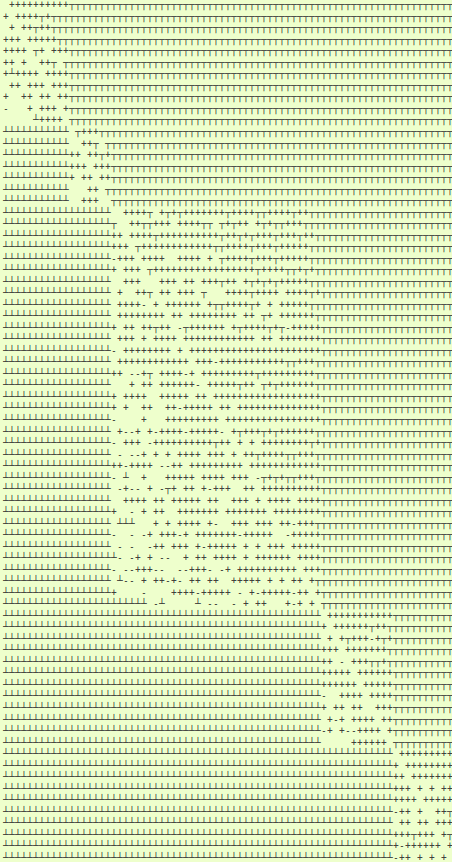
\includegraphics[width=7cm]{Figures/11-1-sparseRelationMap.png}
\caption{Sparse quartiles-sorting decomposed outranking relation (extract). Legend: \emph{outranking} for certain ($\top$); \emph{outranked} for certain ($\bot$); more or less \emph{outranking} ($+$); more or less \emph{outranked} ($-$); \emph{indeterminate}}
\label{fig:11.1}       % Give a unique label
\end{figure}
%\clearpage

With a fill rate of $25\%$, the memory occupation of this sparse outranking digraph \texttt{sg} instance takes now only $769$kB, compared to the $1.7$MB required by a corresponding standard \texttt{BipolarOutrankingDigraph} instance (see List.\vref{list:11.3}).
\begin{lstlisting}
>>> print('%.0fkB' % (total_size(sg)/1024) )
    769kB
\end{lstlisting}

For sparse outranking digraphs, the adjacency table is implemented as a dynamic \texttt{relation()} function instead of a double dictionary.
\begin{lstlisting}[caption={The \texttt{relation()} function of a sparse outranking digraph},label=list:11.4,basicstyle=\ttfamily\scriptsize]
   def relation(self, int x, int y):
       """
       *Parameters*:
           * x (int action key),
           * y (int action key).
       Dynamic construction of the global outranking
       characteristic function *r(x S y)*.
       """
       cdef int Min, Med, Max, rx, ry
       Min = self.valuationdomain['min']
       Med = self.valuationdomain['med']
       Max = self.valuationdomain['max']
       if x == y:
           return Med
       cx = self.actions[x]['component']
       cy = self.actions[y]['component']
       #print(self.components)
       rx = self.components[cx]['rank']
       ry = self.components[cy]['rank']
       if rx == ry:
           try:
               rxpg = self.components[cx]['subGraph'].relation
               return rxpg[x][y]
           except AttributeError:
               componentRanking = self.components[cx]['componentRanking']
               if componentRanking.index(x) < componentRanking.index(x):
                   return Max
               else:
                   return Min
       elif rx > ry:
           return Min
       else:
           return Max
\end{lstlisting}

\section{Quantiles ranking of big performance tableaux}
\label{sec:11.4}

The \texttt{boostedRanking} attribute of the sparse outranking digraph \texttt{sg} contains the global linear ranking of the 100 decision alternatives. This ranking is computed by locally ranking the individual 6 components with the \Copeland rule (see List.~\vref{list:11.3} Lines 12 and 33).
\begin{lstlisting}
>>> sg.boostedRanking
  [22, 53, 3, 34, 56, 62, 24, 44, 50, 93, 41, 63, 29, 58,
   96, 7, 43, 81, 91, 35, 25, 76, 66, 65, 8, 10, 1, 11, 61,
   30, 48, 45, 68, 5, 89, 57, 59, 85, 82, 73, 33, 94, 70,
   97, 20, 92, 71, 90, 95, 21, 28, 2, 36, 87, 40, 98, 46, 55,
   100, 64, 17, 26, 27, 19, 69, 6, 38, 4, 37, 60, 31, 77, 78,
   47, 99, 18, 12, 80, 54, 88, 39, 9, 72, 86, 42, 13, 23, 67,
   52, 15, 32, 49, 51, 74, 16, 14, 75, 79, 83, 84]
\end{lstlisting}

When actually computing linear rankings of the complete set of alternatives, the local outranking relations per component are of no practical usage, and we may furthermore reduce the memory occupation of the resulting digraph by:
\begin{enumerate}[topsep=1pt]
\item refining the ordering of the quantile classes by taking into account how well an alternative is outranking the lower limit of its quantile class, respectively the upper limit of its quantile class is \emph{not} outranking the alternative;
\item dropping the local outranking digraphs and keeping for each component only a locally ranked list of alternatives.
\end{enumerate}

We provide therefore the \texttt{cQuantilesRankingDigraph} class\index{cQuantilesRankingDigraph@\texttt{cQuantilesRankingDigraph} class} from the \texttt{cSparseIntegerOutrankingDigraphs} module.
\begin{lstlisting}[caption={Ranking the sparse integer outranking digraph},label=list:11.5]
>>> from cSparseIntegerOutrankingDigraphs import\
...           cQuantilesRankingDigraph
>>> qr = cQuantilesRankingDigraph(t,4)
>>> qr
 *----- Object instance description --------------*
  Instance class    : cQuantilesRankingDigraph
  Instance name     : cRandomperftab_mp
  Actions           : 100
  Criteria          : 7
  Sorting by        : 4-Tiling
  Ordering strategy : optimal
  Ranking rule      : Copeland
  Components        : 47
  Minimal order     : 1
  Maximal order     : 10
  Average order     : 2.1
  fill rate         : 2.566%
 *----  Constructor run times (in sec.) ----*
  Nbr of threads    : 1
  Total time        : 0.03702
  QuantilesSorting  : 0.01785
  Preordering       : 0.00022
  Decomposing       : 0.01892
  Attributes       : ['runTimes', 'name',
  'actions', 'order', 'dimension', 'sortingParameters',
  'nbrOfCPUs','valuationdomain', 'profiles', 'categories',
  'sorting', 'minimalComponentSize','decomposition',
  'nbrComponents', 'nd', 'components', 'fillRate',
  'maximalComponentSize', 'componentRankingRule', 'boostedRanking']
\end{lstlisting}

With this \emph{optimised} quantile ordering strategy, we obtain now 47 performance equivalence classes (see List.~\vref{list:11.5} Line 13).
\begin{lstlisting}[caption={The ordered components of the sparse outranking digraph},label=list:11.6]
>>> qr.components
    OrderedDict([
    ('c01', {'rank': 1,
	     'lowQtileLimit': ']0.75',
	     'highQtileLimit': '1.00]',
	     'componentRanking': [53]}),
    ('c02', {'rank': 2,
	     'lowQtileLimit': ']0.75',
	     'highQtileLimit': '1.00]',
	     'componentRanking': [3, 23, 63, 50]}),
    ('c03', {'rank': 3,
	     'lowQtileLimit': ']0.75',
	     'highQtileLimit': '1.00]',
	     'componentRanking': [34, 44, 56, 24, 93, 41]}), 
    ...
    ...
    ...
    ('c45', {'rank': 45,
	     'lowQtileLimit': ']0.25',
	     'highQtileLimit': '0.50]',
	     'componentRanking': [49]}),
    ('c46', {'rank': 46,
	     'lowQtileLimit': ']0.25',
	     'highQtileLimit': '0.50]',
	     'componentRanking': [52, 16, 86]}),
    ('c47', {'rank': 47,
	     'lowQtileLimit': ']<',
	     'highQtileLimit': '0.25]',
	     'componentRanking': [79, 83, 84]})])
>>> print('%.0fkB' % (total_size(qr)/1024) )
    208kB
\end{lstlisting}

We observe in Listing~\vref{list:11.6} an even more considerably less voluminous memory occupation 208kB, compared to the 769kB of the \texttt{SparseIntegerOutran\-king\-Digraph} instance.

It is opportune, however, to measure the loss of quality of the resulting \Copeland ranking when working with sparse outranking digraphs.
\begin{lstlisting}[caption={Measuring the loss of quality with respect to the standard outranking digraph},label=list:11.7]
>>> from cIntegerOutrankingDigraphs import\
...                       IntegerBipolarOutrankingDigraph
>>> ig = IntegerBipolarOutrankingDigraph(t)
>>> print('Complete outranking : %+.3f'\
...    % (ig.computeOrderCorrelation(\
...             ig.computeCopelandOrder())['correlation']))
    Complete outranking : +0.747

>>> print('Sparse 4-tiling : %+.3f'\
...     % (ig.computeOrderCorrelation(\
...        list(reversed(sg.boostedRanking)))['correlation']))   
    Sparse 4-tiling          : +0.717

>>> print('Optimzed sparse 4-tiling: %+.3f'\
...  % (ig.computeOrderCorrelation(\
...     list(reversed(qr.boostedRanking)))\
...     ['correlation']))  
    Optimzed sparse 4-tiling: +0.705
\end{lstlisting}

The best ranking correlation with the pairwise outranking situations ($+0.747$) is naturally given when we apply the \Copeland rule to the standard outranking digraph (see List.~\vref{list:10.7} Line 7). When applying the same rule to the sparse 4-tiled outranking digraph, one gets a correlation of $+0.717$ (Line 12), and when applying the \Copeland rule to the optimised sparse 4-tiled digraph, we still obtain a correlation of $+0.705$ (Line 18). These optimistic results actually depend on the number of quantiles we use as well as on the given model of random performance tableau.

In case of \texttt{Random3ObjectivesPerformanceTableau} instances, for instance, we would get in a similar setting an even better standrad outranking correlation of $+0.86$, a sparse 4-tiling correlation of $+0.82$, and an optimised sparse 4-tiling correlation of $+0.81$.

\section{HPC quantiles ranking records}
\label{sec:11.5}

Following from the separability property of the $q$-tiles sorting of each action into a $q$-tiles class, the $q$-sorting algorithm may be safely split into as much threads as are multiple processing cores available for working in parallel (see Prop.~\ref{prop:9.1}). Furthermore, the ranking procedure being local to each diagonal component, these procedures may as well be safely processed in parallel threads on each component restricted outranking digraph.

Using the HPC platform of the University of Luxembourg -- https://hpc-docs.uni.lu/ \citep{UNI-2014}-- the following run times for very big ranking problems could be achieved both on:
\begin{itemize}[topsep=1pt]
\item \emph{Iris -skylake} nodes with 28 cores:\\
  (see \href{https://hpc-docs.uni.lu/systems/iris/}{https://hpc-docs.uni.lu/systems/iris}), and
\item the 3TB -bigmem \emph{Gaia-183} node with 64 cores \\
  (see \href{https://hpc.uni.lu/systems/gaia/}{https://hpc.uni.lu/systems/gaia}),
\end{itemize}
by running the cythonized Python modules in an Intel compiled virtual Python 3.6.5 environment [GCC Intel(R) 17.0.1 –enable-optimizations c++ gcc 6.3 mode] on Debian 8 Linux.

\begin{figure}[ht]
\sidecaption
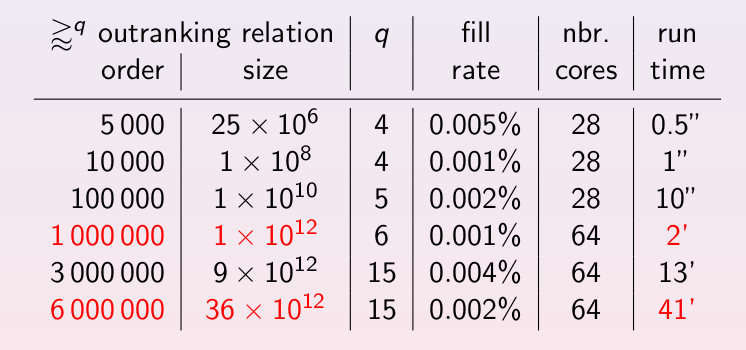
\includegraphics[width=7cm]{Figures/11-2-rankingRecords.png}
\caption{HPC-UL Ranking Performance Records (Spring 2018). On the big memory equipped Gaia-183 node, we were able to rank a million decision alternatives in about 2 minutes. We even could linearly rank up to 6 million decision alternatives in about 40 minutes}
\label{fig:11.2}       % Give a unique label
\end{figure}
  
%%%%%%% The chapter bibliography
%\normallatexbib
%\clearpage
%\phantomsection
%\addcontentsline{toc}{chapter}{Chapter Bibliography}
%\input{02-mainMatters/11-chapterHPCRanking.bbl}
\bibliographystyle{spbasic}
\bibliography{03-backMatters/reference}

\bibliographystyle{spbasic}
\bibliography{03-backMatters/reference}

\bibliographystyle{spbasic}
\bibliography{03-backMatters/reference}

\bibliographystyle{spbasic}
\bibliography{03-backMatters/reference}
